% !TeX program = xelatex
% ------------------------------------------------------------
%  全国大学生数学建模竞赛 论文模板(强化版)
%  适配:题目“C题.pdf”与“人工智能工具使用规定.pdf”的常见要求
%  特点:版面规范、美观易读、图表三线表、符号/缩略语、可复制的模型环境
%  编译:推荐 XeLaTeX(两次)+ 参考文献(手工thebibliography)
% ------------------------------------------------------------
\documentclass[12pt,a4paper]{ctexart}

% --- 基础版式 ---
\usepackage[top=25mm,bottom=25mm,left=25mm,right=25mm,headsep=6mm,headheight=14pt]{geometry}
\usepackage{setspace}
\setstretch{1.25} % 行距 1.25
\usepackage{indentfirst}
\setlength{\parindent}{2em}
\usepackage{titlesec}
\titleformat{\section}{\bfseries\Large}{\thesection.}{0.6em}{}
\titleformat{\subsection}{\bfseries\large}{\thesubsection}{0.6em}{}
\titleformat{\subsubsection}{\bfseries}{\thesubsubsection}{0.6em}{}
\ctexset{today=small}

% --- 页眉页脚 ---
\usepackage{fancyhdr}
\pagestyle{fancy}
\fancyhf{}
\fancyhead[L]{全国大学生数学建模竞赛论文}
\fancyhead[R]{\thepage}
\renewcommand{\headrulewidth}{0.4pt}

% --- 数学与符号 ---
\usepackage{amsmath,amssymb,amsfonts,bm,mathtools}
\numberwithin{equation}{section}
\usepackage{siunitx}
\sisetup{group-minimum-digits=4,round-mode=places,round-precision=3}
\usepackage{amsmath}
\usepackage{amssymb}  
% --- 图表 ---
\usepackage{graphicx}
\usepackage{float}
\usepackage{subcaption}
\usepackage{booktabs,threeparttable,multirow,tabularx,longtable}
\renewcommand{\arraystretch}{1.18}
\usepackage{cancel}
% 三线表统一样式
\newcommand{\toprulethick}{\specialrule{1pt}{1pt}{1pt}}
\newcommand{\midrulethin}{\specialrule{0.5pt}{0pt}{0pt}}
\newcommand{\bottomrulethick}{\specialrule{1pt}{1pt}{1pt}}
\usepackage[labelfont=bf,labelsep=quad]{caption}
\captionsetup{font=small}

% --- 代码/算法(如需要) ---
\usepackage{listings}
\lstset{basicstyle=\ttfamily\small,breaklines=true,frame=single,backgroundcolor=\color[gray]{0.97}}
\usepackage[ruled,vlined,linesnumbered]{algorithm2e}
\SetKwInput{KwIn}{输入}
\SetKwInput{KwOut}{输出}

% --- 颜色 & 超链接 ---
\usepackage{xcolor}
\definecolor{linkblue}{RGB}{0,70,140}
\usepackage[colorlinks=true,linkcolor=linkblue,citecolor=linkblue,urlcolor=linkblue]{hyperref}

% --- 自定义环境:模型/假设/结论等 ---
\usepackage{amsthm}
\newtheoremstyle{mcm}% name
{0.5em}% Space above
{0.5em}% Space below
{\itshape}% Body font
{}% Indent amount
{\bfseries}% Theorem head font
{.}% Punctuation after theorem head
{0.5em}% Space after theorem head
{}
\theoremstyle{mcm}
\newtheorem{assump}{假设}[section]
\newtheorem{defn}{定义}[section]
\newtheorem{prop}{命题}[section]
\newtheorem{thm}{定理}[section]

% --- 常用符号宏 ---
\newcommand{\E}{\mathbb{E}}
\newcommand{\Var}{\mathrm{Var}}
\newcommand{\Cov}{\mathrm{Cov}}
\newcommand{\argmin}{\mathop{\mathrm{arg\,min}}\limits}
\newcommand{\argmax}{\mathop{\mathrm{arg\,max}}\limits}

% --- 封面(可按赛题需求替换为匿名/队号版) ---
\newcommand{\papertitle}{基于层级回归的NIPT Y染色体浓度影响因素研究}
\newcommand{\teamid}{XXXXXX} % 队号(如需)

\begin{document}

% ================= 封面 =================
\begin{titlepage}
  \centering
  {\heiti\zihao{2} 全国大学生数学建模竞赛论文}\par\vspace{24pt}
  {\bfseries\zihao{2} \papertitle}\par\vspace{18pt}
  {\zihao{-3}(题目:C题)}\par\vspace{24pt}
  {\zihao{-3} 队号:\teamid}\par\vfill
  {\today}
\end{titlepage}
\setcounter{page}{1}

% ================= 摘要与关键词 =================
\begin{abstract}
为匹配竞赛评审的阅读习惯,摘要建议控制在\SI{300}{\text{--}\,400}字,交代:问题目标、关键方法(如混合效应模型/广义线性模型/优化求解等)、核心结论与指标(R\textsuperscript{2}、MAE、鲁棒性检验)、应用价值与推广。英文摘要可在附录给出。
\end{abstract}
\textbf{关键词:}NIPT;混合效应模型;二次多项式;变量变换;模型检验

% ================= 1 问题背景与重述 =================
\section{问题背景与重述}

\subsection{问题背景}
无创产前检测(Non-invasive Prenatal Test, NIPT)是一项前沿的产前筛查技术,它通过采集孕妇的静脉血,提取其中包含的胎儿游离DNA片段(cffDNA),并对其进行高通量测序和生物信息学分析,从而评估胎儿患上染色体非整倍体疾病的风险。临床上,NIPT主要用于检测三种最常见的染色体异常疾病:唐氏综合征(21号染色体三体)、爱德华氏综合征(18号染色体三体)和帕陶氏综合征(13号染色体三体)。

NIPT检测的准确性在很大程度上取决于胎儿游离DNA在母体血浆中的浓度,即胎儿分数。对于男胎而言,Y染色体浓度是一个关键的质量控制指标。通常认为,当男胎的Y染色体浓度达到或超过4\%时,检测结果才具有较高的可靠性。然而,胎儿的Y染色体浓度受到多种因素的共同影响,其中孕妇的孕周(Gestational Age)和身体质量指数(Body Mass Index, BMI)被证实是两个核心相关因素。

在临床实践中,选择合适的NIPT检测时点至关重要。过早检测可能因胎儿分数不足而导致测序失败或结果不准确;而过晚检测则可能错失最佳的临床干预窗口,从而增加孕妇及其家庭的风险。早期(12周内)发现异常的风险较低,而中晚期(13周后)发现则风险显著增高。由于不同孕妇在年龄、BMI、孕情等方面存在显著的个体差异,采用统一的检测时点方案难以满足个性化的需求,可能影响检测的整体效能。因此,如何根据孕妇的个体特征(特别是BMI)进行科学分组,并为每个群体确定最佳的NIPT检测时点,以实现风险最小化,是当前产前诊断领域亟待解决的一个重要问题。

\subsection{赛题重述}
本研究旨在利用提供的孕妇NIPT检测数据,建立数学模型来解决NIPT时点选择与胎儿异常判定的相关问题。具体任务如下:
\begin{enumerate}
    \item \textbf{相关性分析与建模:} 分析胎儿染色体浓度与孕妇的孕周、BMI等关键指标之间的相关特性,建立能够描述它们之间关系的数学模型,并对模型的显著性进行检验。
    \item \textbf{基于BMI的男胎NIPT时点优化:} 临床研究表明,BMI是影响男胎Y染色体浓度最早达标时间的主要因素。要求对男胎孕妇根据BMI进行合理分组,确定每个分组的BMI区间和最佳NIPT检测时点,目标是使孕妇因延迟诊断而面临的潜在风险最小化,并分析检测误差对结果可能产生的影响。
    \item \textbf{多因素下男胎NIPT时点优化:} 在问题二的基础上,进一步综合考虑孕妇的身高、体重、年龄等多种因素,结合检测误差和Y染色体浓度达标比例,为不同BMI分组的男胎孕妇设计更为精细的最佳NIPT时点方案,并对潜在风险和检测误差的影响进行分析。
    \item \textbf{女胎异常判定方法构建:} 由于女胎不含Y染色体,其异常判定需依赖其他生物信息学指标。要求以已知的21、18、13号染色体非整倍体检测结果为标准,综合运用X染色体及上述染色体的Z值、GC含量、读段数、孕妇BMI等多种信息,构建一个科学、可靠的女胎染色体异常判定方法。
\end{enumerate}



提炼\textbf{四个问题}的具体目标、输入输出与评判标准,给出流程图(图~\ref{fig:flow})。
\begin{figure}[H]
  \centering
  % \includegraphics[width=0.85\linewidth]{figs/flowchart.pdf}
  \caption{整体求解流程示意}
  \label{fig:flow}
\end{figure}

% ================= 2 问题分析 =================
\section{问题分析}
从数据统计特征、变量相关性与共线性、重复测量结构(“孕妇代码”)与噪声来源三个层面分析。可给出皮尔逊/斯皮尔曼相关矩阵热力图,并讨论为何\textbf{层级/混合}框架优于普通回归。

% ================= 3 模型假设 =================
\section{模型假设}
以条目形式给出:观测独立性(条件于个体随机效应)、变量测量误差可忽略、响应变量取值范围与变换的合理性等。示例:
\begin{assump}[数据来源可靠]
数据来源可靠且具有代表性,测量的 Y 染色体浓度无严重系统误差。
\end{assump}
\begin{assump}[层级独立]
条件于个体随机效应$u_i\sim\mathcal{N}(0,\sigma_u^2)$时,同一孕妇不同检测的误差$\varepsilon_{ij}$相互独立,且$\varepsilon_{ij}\sim\mathcal{N}(0,\sigma_e^2)$。
\end{assump}
\begin{assump}[簇独立性]
同一孕妇的多次检测构成一个"簇",簇内观测相关但簇间相互独立。
\end{assump}
\begin{assump}[随机截距]
个体差异主要体现在基线水平上,可用随机截距刻画;随机截距 \( u_i \sim \mathcal{N}(0, \sigma_u^2) \)。
\end{assump}
\begin{assump}[残差独立性]
条件于协变量后,残差 \( \epsilon_{ij} \sim \mathcal{N}(0, \sigma^2) \),且与 \( u_i \) 独立。
\end{assump}
\begin{assump}[响应变量变换]
\( Y \) 为比例/分数型时,采用 \( Y_t = \arcsin{\sqrt{Y}} \) 变换以改善方差稳定性与正态性(工程近似)。
\end{assump}
\begin{assump}[潜在因素影响可忽略]
除选取的主要自变量外,其它潜在因素的影响可忽略,或已被随机效应
吸收。
\end{assump}
\begin{assump}[风险连续性]
检测延迟带来的风险是连续增长的,符合二次函数规律
\end{assump}
\begin{assump}[重测]
检测失败后需要重新检测
\end{assump}
\begin{assump}[时间序列展开]
个体观测记录可展开为逐周时间序列,风险在0.5周间隔内恒定,首次达标后保持达标状态。
\end{assump}
\begin{assump}[连续风险函数]
存在连续危险度函数 \( h(t|X) \),协变量影响为乘性,个体间风险独立。
\end{assump}
\begin{assump}[样条平滑建模]
孕周和BMI影响可通过自然样条平滑建模,存在交互效应,年龄影响非线性。
\end{assump}
\begin{assump}[排序稳定性]
同个体不同时间点风险排序稳定,同受试者样本组内排序,NDCG优化提升排序质量。
\end{assump}
\begin{assump}[分层独立校准]
BMI和孕周分层内概率校准独立,校准函数单调,不改变原始排序关系。
\end{assump}
\begin{assump}[组内相关性]
同受试者不同时间点样本相关,不同受试者样本独立,分组交叉验证处理时间依赖。
\end{assump}
\begin{assump}[临床阈值固定]
 Y染色体浓度 \( \geq 4\% \) 为检测准确性关键阈值,BMI为主要影响因素,早期检测提供更长治疗窗口。
\end{assump}
\begin{assump}[排序学习优势]
排序学习比传统分类更适合不平衡时间序列数据,模型集成提供稳健预测,BMI和孕周为重要特征。
\end{assump}
\begin{assump}[函数平滑性]
风险函数平滑,协变量效应线性,校准函数单调,在大多数情况下成立。
\end{assump}
\begin{assump}[样本不平衡]
标签定义以“否/异常/阳性/不健康”为正类,正类稀少,样本极不平衡。
\end{assump}
\begin{assump}[优化目标]
以最大化 PR-AUC 为主目标,ROC-AUC 为辅。
\end{assump}
\begin{assump}[概率校准]
输出的 \( \hat{p}(x) \) 需能反映真实发生率,用等渗回归进行概率校准。
\end{assump}


% ================= 4 符号说明 =================
\section{符号说明}
\begin{longtable}{p{0.18\textwidth}p{0.74\textwidth}}
\toprulethick
符号 & 含义 \\
\midrulethin
$y_{ij}$ & 第$i$位孕妇第$j$次检测的Y染色体浓度(或其变换)。\\
$\text{GA}_{ij}$、$\text{BMI}_{ij}$ & 孕周、BMI;$\text{GA}_c=\text{GA}-\overline{\text{GA}}$ 等中心化量。\\
$\text{HasPrev}_i$ & 既往妊娠指示变量(0/1)。\\
$u_i$ & 个体随机截距;$u_i\sim\mathcal{N}(0,\sigma_u^2)$。\\
$\varepsilon_{ij}$ & 条件误差;$\varepsilon_{ij}\sim\mathcal{N}(0,\sigma_e^2)$。\\
\( x \in \mathbb{R}^d \) & 特征向量(年龄、孕周、BMI、测序质控、X/Y 浓度、Z 值等) \\
\( y \in \{0,1\} \) & 标签(1=异常) \\
\( f_{\text{RF}}(\cdot) \) & 随机森林分类器(多数投票) \\
\( \hat{p}(x) \) & 校准后的异常概率(isotonic) \\
\( \tau \) & 判定阈值(0.5 / Best-F1 / 召回≥80\% 的最优阈) \\
PR-AUC(AP) & 精确率-召回曲线下的面积 \\
Brier & 概率预测的均方误差 \\
CM & 混淆矩阵(TP/FP/FN/TN) \\
\( i = 1, \ldots, G \) & 孕妇(簇)编号 \\
\( j = 1, \ldots, n_i \) & 第 \( i \) 位孕妇的第 \( j \) 次检测 \\
\( Y_{ij} \) & 第 \( i \) 位孕妇第 \( j \) 次的 Y 染色体浓度(或胎儿分数) \\
\( Y_{ij}^{(t)} \) & 变换后的响应 \( \arcsin \sqrt{Y_{ij}} \) \\
\(GA_c, BMI_c\) & 孕周/BMI 的中心化变量 \\
HasPrevPreg & 既往妊娠指示变量(0/1) \\
\( u_i \) & 孕妇 \( i \) 的随机截距,\( u_i \sim \mathcal{N}(0, \sigma_u^2) \) \\
\( \varepsilon_{ij} \) & 条件残差,\( \varepsilon_{ij} \sim \mathcal{N}(0, \sigma^2) \)\\
ICC & 簇内相关:\( \sigma_u^2/(\sigma_u^2 + \sigma^2) \) \\
\( R_m^2, R_c^2 \) & 混合模型的边际/条件 \( R^2 \)(Nakagawa \& Schielzeth) \\
\( Y \) & Y染色体浓度(胎儿游离DNA中Y比例)  \\
\( Y^* \) & 变换后的浓度,\( Y^* = \arcsin(\sqrt{Y}) \)  \\
\( s_i \) & 个体标识符(孕妇\( i \)) \\
\( t_i, t_{i,j} \) & 孕周及其观测值 \\
\( \text{bmi}_i \) & 体重指数  \\
\( \text{age}_i \) & 年龄  \\
\bottomrulethick
\end{longtable}
\begin{longtable}{p{0.18\textwidth}p{0.74\textwidth}}
\toprulethick
符号 & 含义 \\
\midrule
\( y_i, y_{i,j} \) & 事件指示变量,\( y_i = 1 \)当且仅当\( Y \geq 4\% \)  \\
\( x_i \) & 协变量向量,\( x_i = (\text{bmi}_i, \text{age}_i, \text{height}_i, \text{weight}_i) \) \\
\( X \) & 设计矩阵,\( X \in \mathbb{R}^{n \times p} \)  \\
\( B_t(t) \) & 周样条基函数  \\
\( B_{\text{bmi}}(\text{bmi}) \) & BMI样条基函数  \\
\( B_{\text{int}}(t, \text{bmi}) \) & 交互项样条基函数  \\
\( k_t \) & 周样条结点集合 \\
\( k_{\text{bmi}} \) & BMI样条结点集合  \\
\( f(x) \) & 排序函数,\( f : \mathbb{R}^p \to \mathbb{R} \)  \\
\( \cancel{C}_{\text{rank}} \) & LambdaRank排序损失函数 \\
\( \lambda_{ij} \) & Lambda梯度 \\
\( G_i \) & 个体\( s_i \)的样本组  \\
\( \text{NDCG}_{ij} \) & 归一化折扣累积增益  \\
\( g_s(p) \) & 层\( s \)的单调映射函数  \\
\( p_{\text{cal}} \) & 校准后的概率 \\
\( T \) & 温度参数 \\
\( h(t|\text{bmi}) \) & 危险度函数 \\
\( t^*(\text{bmi}) \) & 最优检测时机函数  \\
\( E[R(t, \text{bmi})] \) & 期望风险函数  \\
AUC & ROC曲线下面积  \\
PR-AUC & PR曲线下面积 \\
ECE & 期望校准误差  \\
\( \alpha, \beta \) & 校准斜率和截距  \\
\bottomrulethick
\end{longtable}

% ================= 5 数据处理与分析 =================
\section{数据处理与分析}
\subsection{基础清理}
删除空列
\subsection{缺失值统计分析}
本文对数据中的缺失值进行了详细分析,分别对男性和女性数据的缺失情况进行了统计,结果如下图所示。
% \begin{figure}[htbp]
%     \centering
%     \begin{subfigure}{0.45\textwidth}
%         \includegraphics[width=\linewidth]{code/论文/missing_male.png}
%         \caption{男胎缺失值分析}
%     \end{subfigure}
%     \hfill
%     \begin{subfigure}{0.45\textwidth}
%         \includegraphics[width=\linewidth]{code/论文/missing_female.png}
%         \caption{女胎缺失值分析}
%     \end{subfigure}
%     \caption{缺失值统计分析}
%     \label{fig:missing_analysis}
% \end{figure}
\subsection{孕周数据处理}
根据末次月经日期和检测日期计算孕周天数,比较与原始数据中的孕周是否一致,统计差异情况
\begin{figure}[htbp]
    \centering
    \begin{subfigure}{0.45\textwidth}
        \includegraphics[width=\linewidth]{code/论文/gestation_compare_male.png}
        \caption{男胎}
    \end{subfigure}
    \hfill
    \begin{subfigure}{0.45\textwidth}
        \includegraphics[width=\linewidth]{code/论文/gestation_compare_female.png}
        \caption{女胎}
    \end{subfigure}
    \caption{孕周数据差异统计}
    \label{fig:missing_analysis}
\end{figure}
\subsection{BMI数据处理}
根据身高体重计算BMI值,比较与原始数据中的BMI是否一致,统计差异情况
\begin{figure}[htbp]
    \centering
    \begin{subfigure}{0.45\textwidth}
        \includegraphics[width=\linewidth]{code/论文/bmi_compare_female.png}
        \caption{女胎}
    \end{subfigure}
    \hfill
    \begin{subfigure}{0.45\textwidth}
        \includegraphics[width=\linewidth]{code/论文/bmi_compare_male.png}
        \caption{男胎}
    \end{subfigure}
    \caption{BMI数据差异统计}
    \label{fig:missing_analysis}
\end{figure}
\subsection{特征工程}
将"自然受孕/IUI/IVF"等文本映射为数值(0/1/2),便于建模
\subsection{数据剔除}
缺失行剔除:删除原始列中有缺失值的行;GC离群值剔除:使用Tukey IQR方法剔除GC含量异常低的样本(仅下界剔除)。
\begin{figure}[htbp]
    \centering
    \begin{subfigure}{0.9\textwidth}
        \includegraphics[width=\linewidth]{code/论文/exclusion_report_female.png}
        \caption{女胎}
    \end{subfigure}
    \hfill
    \begin{subfigure}{0.9\textwidth}
        \includegraphics[width=\linewidth]{code/论文/exclusion_report_male.png}
        \caption{男胎}
    \end{subfigure}
    \caption{数据剔除情况}
    \label{fig:missing_analysis}
\end{figure}
\subsection{数据总览与相关性分析}
分析数据相关性,通过相关性热图可视化
\begin{figure}[htbp]\centering
    \includegraphics[width=0.5\linewidth]{code/论文/aa06c72d7d6e442294f5a57c8cf5e46e.png}
    \caption{相关性热图}
    \label{fig:missing_analysis}
\end{figure}
\subsection{最终数据导出}
将处理后的数据保存为UTF-8编码的CSV文件,供后续建模使用
% ================= 6 模型建立与求解 =================
\section{模型建立与求解}
\subsection{问题一的模型建立与求解}
{\begingroup
  \setcounter{secnumdepth}{3} % 确保 \subsubsection 有编号
  % ✦ 关键:先缓存“原版”的 \subsubsection
  \let\SavedSubsubsection\subsubsection
  % 让 \subsection 映射到“原版 \subsubsection”(会产生 6.1.1、6.1.2 …)
  \renewcommand{\subsection}{\SavedSubsubsection}
  % 再把 \subsubsection 降一级为 \paragraph(通常无编号)
  \renewcommand{\subsubsection}{\paragraph}

\subsection{单因素探索(Exploratory Analysis)}
为判断是否需要非线性项并初步识别方向性,我们对孕周(GA)与体重指数(BMI)分别与 $Y$ 浓度做了散点与斯皮尔曼相关(Spearman correlation)探索。图~\ref{fig:ga_scatter} 显示 $Y$ 随孕周整体呈缓慢上升趋势(标题内含 $r$ 与 $p$ 值),提示可考虑加入二次项以刻画轻微曲率;图~\ref{fig:bmi_scatter} 显示 $Y$ 与 BMI 为弱负相关($r<0$),形状近似线性,但为稳妥起见仍纳入二次项以便模型选择阶段检验其必要性。

\begin{figure}[H]\centering
  \begin{subfigure}[t]{.48\linewidth}
    \includegraphics[width=\linewidth]{scatter_Y_vs_GA.png}
    \caption{$Y$ 浓度 vs. 孕周(GA)的单因素关系。}
    \label{fig:ga_scatter}
  \end{subfigure}\hfill%
  \begin{subfigure}[t]{.48\linewidth}
    \includegraphics[width=\linewidth]{scatter_Y_vs_BMI.png}
    \caption{$Y$ 浓度 vs. 体重指数(BMI)的单因素关系。}
    \label{fig:bmi_scatter}
  \end{subfigure}
  \caption{单因素探索:$Y$ 与 GA / BMI 的关系}
  \label{fig:q1_single_factor_pair}
\end{figure}


\subsection{变量变换与预处理(Transformation \& Preprocessing)}
$Y$ 为比例型变量、在 $[0,1]$ 内且偏零。为改善方差稳定性与近似正态,我们采用经典的
\[
  Y^{*}=\arcsin\!\big(\sqrt{Y}\big)
\]
作为响应(方差稳定化变换)。连续自变量统一做\emph{均值中心化}(记后缀 \(_c\)),并为每个连续变量引入二次项(记后缀 \(^2\)),以捕捉潜在弯曲效应并减小与一次项的共线性。二分类变量“是否有既往妊娠(Has previous pregnancy)”按 0/1 处理。

\subsection{候选结构与最终模型(Model Family \& Final Form)}
考虑“同一孕妇多次检测”的重复测量特征,我们采用\textbf{线性混合效应模型}(Linear Mixed-Effects Model, LMM),以\textbf{随机截距}刻画个体基线差异。经基于极大似然(ML)的 AICc/似然比检验对固定效应逐步比较后,最终选择的\emph{多元二次}固定效应集合为(无交互):
\[
\{\text{GA}_c,\text{BMI}_c,\text{Xconc}_c,\text{BTimes}_c,\text{Age}_c,\text{Ht}_c,\text{Wt}_c,\text{GC}_c\}
\quad\text{及其二次项}\quad
\{\text{GA}_c^2,\ldots,\text{GC}_c^2\},
\]
并包含指示变量 \(\mathrm{HasPrevPreg}\)。模型在变换尺度上的数学表达为
\begin{equation}
\label{eq:final_lmm}
\begin{aligned}
Y^{*}_{ij} \;=\;& \beta_0 
 + \beta_1\,\mathrm{GA}_{c,ij} + \beta_2\,\mathrm{GA}_{c,ij}^{2}
 + \beta_3\,\mathrm{BMI}_{c,ij} + \beta_4\,\mathrm{BMI}_{c,ij}^{2}
 + \beta_5\,\mathrm{Xconc}_{c,ij} + \beta_6\,\mathrm{Xconc}_{c,ij}^{2} \\
&+ \beta_7\,\mathrm{BTimes}_{c,ij} + \beta_8\,\mathrm{BTimes}_{c,ij}^{2}
 + \beta_9\,\mathrm{Age}_{c,ij} + \beta_{10}\,\mathrm{Age}_{c,ij}^{2}
 + \beta_{11}\,\mathrm{Ht}_{c,ij} + \beta_{12}\,\mathrm{Ht}_{c,ij}^{2} \\
&+ \beta_{13}\,\mathrm{Wt}_{c,ij} + \beta_{14}\,\mathrm{Wt}_{c,ij}^{2}
 + \beta_{15}\,\mathrm{GC}_{c,ij} + \beta_{16}\,\mathrm{GC}_{c,ij}^{2}
 + \beta_{17}\,\mathrm{HasPrevPreg}_{i} \\
&+\, u_i + \varepsilon_{ij}, 
\qquad u_i\sim\mathcal{N}(0,\sigma_u^2),\quad \varepsilon_{ij}\sim\mathcal{N}(0,\sigma^2),
\end{aligned}
\end{equation}
其中 \(i\) 表孕妇、\(j\) 表同一孕妇的不同检测;\(u_i\) 为个体随机截距。

\subsection{参数估计与实现(Estimation \& Implementation)}
为获得方差成分更稳健的不偏估计,最终模型采用\textbf{限制性最大似然}(Restricted Maximum Likelihood, REML)估计;固定效应的比较阶段使用 ML。实现基于 \texttt{Python/statsmodels} 的 \texttt{MixedLM}。本题数据的 REML 对数似然为
\(\text{logLik}=1407.32\),随机截距方差与残差方差分别估计为
\(\widehat{\sigma_u^2}=0.001906\) 与 \(\widehat{\sigma^2}=0.000716\)。

\subsection{结果与解释(Results \& Interpretation)}
按照 Nakagawa \& Schielzeth(2013/2017)的框架,我们报告两类判定系数:\textbf{边际 \(R^2\)}(Marginal \(R^2\),仅固定效应)与\textbf{条件 \(R^2\)}(Conditional \(R^2\),固定+随机效应)。本模型得到
\[
R^2_\text{marginal}=0.343,\qquad
R^2_\text{conditional}=0.821.
\]
组内相关系数(Intraclass Correlation Coefficient, ICC)
\[
\mathrm{ICC}=\frac{\widehat{\sigma_u^2}}{\widehat{\sigma_u^2}+\widehat{\sigma^2}}
=0.7269,
\]
表明跨孕妇的基线差异占总变异的主要部分;引入随机截距是必要且有效的。系数方向与单因素探索一致:GA 效应总体为正且存在轻微曲率;BMI 的一次项为负更显著,二次项用于捕捉可能的轻度非线性;其余质量/体征变量(Xconc/BTimes/Age/Ht/Wt/GC)的二次项为模型在边际 \(R^2\) 提升提供了补充解释力。

\subsection{模型诊断与稳健性(Diagnostics \& Robustness)}
图~\ref{fig:residfit} 为“残差—拟合值”图,点云在零线附近均匀分布、未见明显漏斗形,支持同方差性;图~\ref{fig:qqplot} 为条件残差的正态 Q--Q 图,大部分点贴近 $45^\circ$ 线,仅上尾有少量偏离,说明正态性基本成立。对潜在异常观测执行删一(leave-one-out)稳健检查,关键系数与 \(R^2\) 变化均较小,结论稳定。

\begin{figure}[H]\centering
  \begin{subfigure}[t]{.48\linewidth}
    \includegraphics[width=\linewidth]{resid_vs_fitted.png}
    \caption{条件残差—拟合值关系图(变换尺度)。}
    \label{fig:residfit}
  \end{subfigure}\hfill%
  \begin{subfigure}[t]{.48\linewidth}
    \includegraphics[width=\linewidth]{qq.png}
    \caption{条件残差的正态 Q--Q 图。}
    \label{fig:qqplot}
  \end{subfigure}
  \caption{模型诊断图:残差—拟合与 Q--Q 并排对比}
  \label{fig:q1_diag_pair}
\end{figure}


\subsection{小结(Summary)}
本题在方差稳定化与中心化二次项的框架下,构建了包含\emph{八个连续协变量的一次与二次项 + 既往妊娠指示}的多元二次 LMM,并以随机截距吸收孕妇间的巨大个体差异。模型在边际/条件 \(R^2\) 与诊断图上均表现良好,能够用于解释与预测变换尺度下的 \(Y\) 浓度;若用于原尺度展示,可将 \(\hat Y^{*}\) 逆变换为 \(\hat Y=\sin^2(\hat Y^{*})\) 以给出直观比例值。
\endgroup}
\subsection{问题二的模型建立与求解}

问题二的核心目标是,针对接受无创产前检测(NIPT)的孕妇,依据其身体质量指数(BMI)进行合理分组,并为每个分组推荐一个最佳的检测时点(以孕周计)。这一策略旨在最小化因检测时点选择不当而引发的综合风险,例如过早检测导致的失败率增高,或因推迟检测而错过了最佳干预时机。

为实现此目标,我们构建了一个从概率建模到优化决策的完整分析框架。首先,我们建立一个概率模型来预测在不同BMI和孕周条件下,Y染色体浓度检测的达标可能性。其次,我们定义一个能够量化潜在风险的期望风险函数。最后,通过优化算法,我们寻找能够使全体孕妇总期望风险最小化的BMI分组方案与相应的推荐检测周。

\subsubsection{模型基础:基于样条回归的达标概率预测}

为了精确描述Y染色体浓度是否达标与孕妇生理特征(尤其是BMI和孕周)之间的复杂关系,我们构建了一个基于改进样条回归的概率预测模型。该模型直接对"是否达标"这一二元结果进行建模,能够有效捕捉非线性趋势。

\paragraph{1. 特征工程与模型设定}
模型的预测效果在很大程度上依赖于特征的构造。我们引入了样条特征来增强模型的表达能力,具体包含了以下部分:
\begin{itemize}
    \item \textbf{基础线性项}:涵盖了标准化处理后的BMI、孕周和年龄。
    \item \textbf{高次项与交互项}:为捕捉变量间的非线性关系,我们加入了$\text{BMI}^2$、$\text{孕周}^2$以及BMI与孕周的交互项(BMI $\times$ 孕周)。
    \item \textbf{二次样条项}:为了更灵活地拟合局部变化趋势,我们分别为BMI和孕周设置了二次样条,形式为$\max(0, \text{变量} - k)^2$,其中$k$是根据数据分位数确定的节点。
\end{itemize}

\paragraph{2. 正则化逻辑回归}
在构建好特征矩阵$\mathbf{X}$后,我们采用带弹性网络正则化(Elastic Net)的逻辑回归模型来拟合达标概率$p$。其基本形式为:
\begin{equation}
    \log\left(\frac{p}{1-p}\right) = \mathbf{X}\boldsymbol{\beta}
\end{equation}
模型的优化目标是在最小化负对数似然损失的同时,对系数$\boldsymbol{\beta}$施加L1和L2范数惩罚,其目标函数如下:
\begin{equation}
    \min_{\boldsymbol{\beta}} \left\{ -\sum_{i=1}^n \left[ y_i \log p_i + (1-y_i) \log(1-p_i) \right] + \lambda_1 \|\boldsymbol{\beta}\|_1 + \lambda_2 \|\boldsymbol{\beta}\|_2^2 \right\}
\end{equation}
这种方法不仅能自适应地捕捉数据中的非线性模式,还能通过正则化有效防止模型过拟合,为后续的风险评估与优化决策提供了稳健的概率预测基础。

我们通过ROC曲线对模型性能进行了评估,其AUC值为0.693,表明该概率模型具有良好的分类预测能力。图~\ref{fig:qualification_probability}直观展示了达标概率在BMI-孕周平面上的分布情况,清晰地揭示了达标可能性随这两个核心变量的变化趋势。

\subsubsection{期望风险最小化模型}

为了对检测时点选择的优劣进行量化评估,我们构建了一个期望风险模型。

\paragraph{1. 风险函数的定义}
我们认为,检测时点带来的风险并非线性增加,也非阶梯式跳跃。因此,我们设计了一个平滑的二次函数来描述风险随检测时点$T$的变化。该函数在孕周11周前风险为最低值$R_{\min}$,在28周后达到最高值$R_{\max}$,中间则平滑过渡。其数学表达式为:
\begin{equation}
    R(T) = 
    \begin{cases} 
        R_{\min} & \text{if } T \le 11 \\
        R_{\min} + a(T - 11)^2 & \text{if } 11 < T < 28 \\
        R_{\max} & \text{if } T \ge 28 
    \end{cases}
\end{equation}
其中,$R_{\min} = 1.0$,$R_{\max} = 30.0$,$a = \frac{R_{\max} - R_{\min}}{(28-11)^2}$。这样的设计既符合风险随时间推移而加速增长的临床直觉,也保证了函数在边界点的连续性,有利于后续的数值优化。

\paragraph{2. 增强的期望风险函数}
传统的期望风险模型通常只考虑检测成功的情况。我们对其进行了改进,引入了检测失败的惩罚机制。对于一位特定BMI的孕妇,在孕周$T$进行检测的期望风险$E(T | \text{BMI})$被定义为:
\begin{equation}
    E(T | \text{BMI}) = p(\text{BMI}, T) \cdot R(T) + (1 - p(\text{BMI}, T)) \cdot [R(T+k) + P_{\text{failure}}]
\end{equation}
此处的$p(\text{BMI}, T)$是由前述样条回归模型预测的达标概率。当检测成功(概率为$p$)时,风险为$R(T)$;当检测失败(概率为$1-p$)时,孕妇不仅要承担下一次检测(假设在$k$周后)的风险$R(T+k)$,还需承受一个额外的失败惩罚$P_{\text{failure}}$(我们设定$k=2$周,$P_{\text{failure}}=10.0$)。这个增强模型更真实地反映了检测失败所带来的时间、经济和心理等多重代价,使优化过程更倾向于选择成功率高且时间较早的检测方案。

图~\ref{fig:expected_risk_heatmap}通过热力图的形式,展示了期望风险在BMI与孕周构成的二维平面上的分布,为后续寻找最优策略提供了直观依据。

\begin{figure}[htbp]
    \centering
    \begin{minipage}{0.48\textwidth}
        \centering
        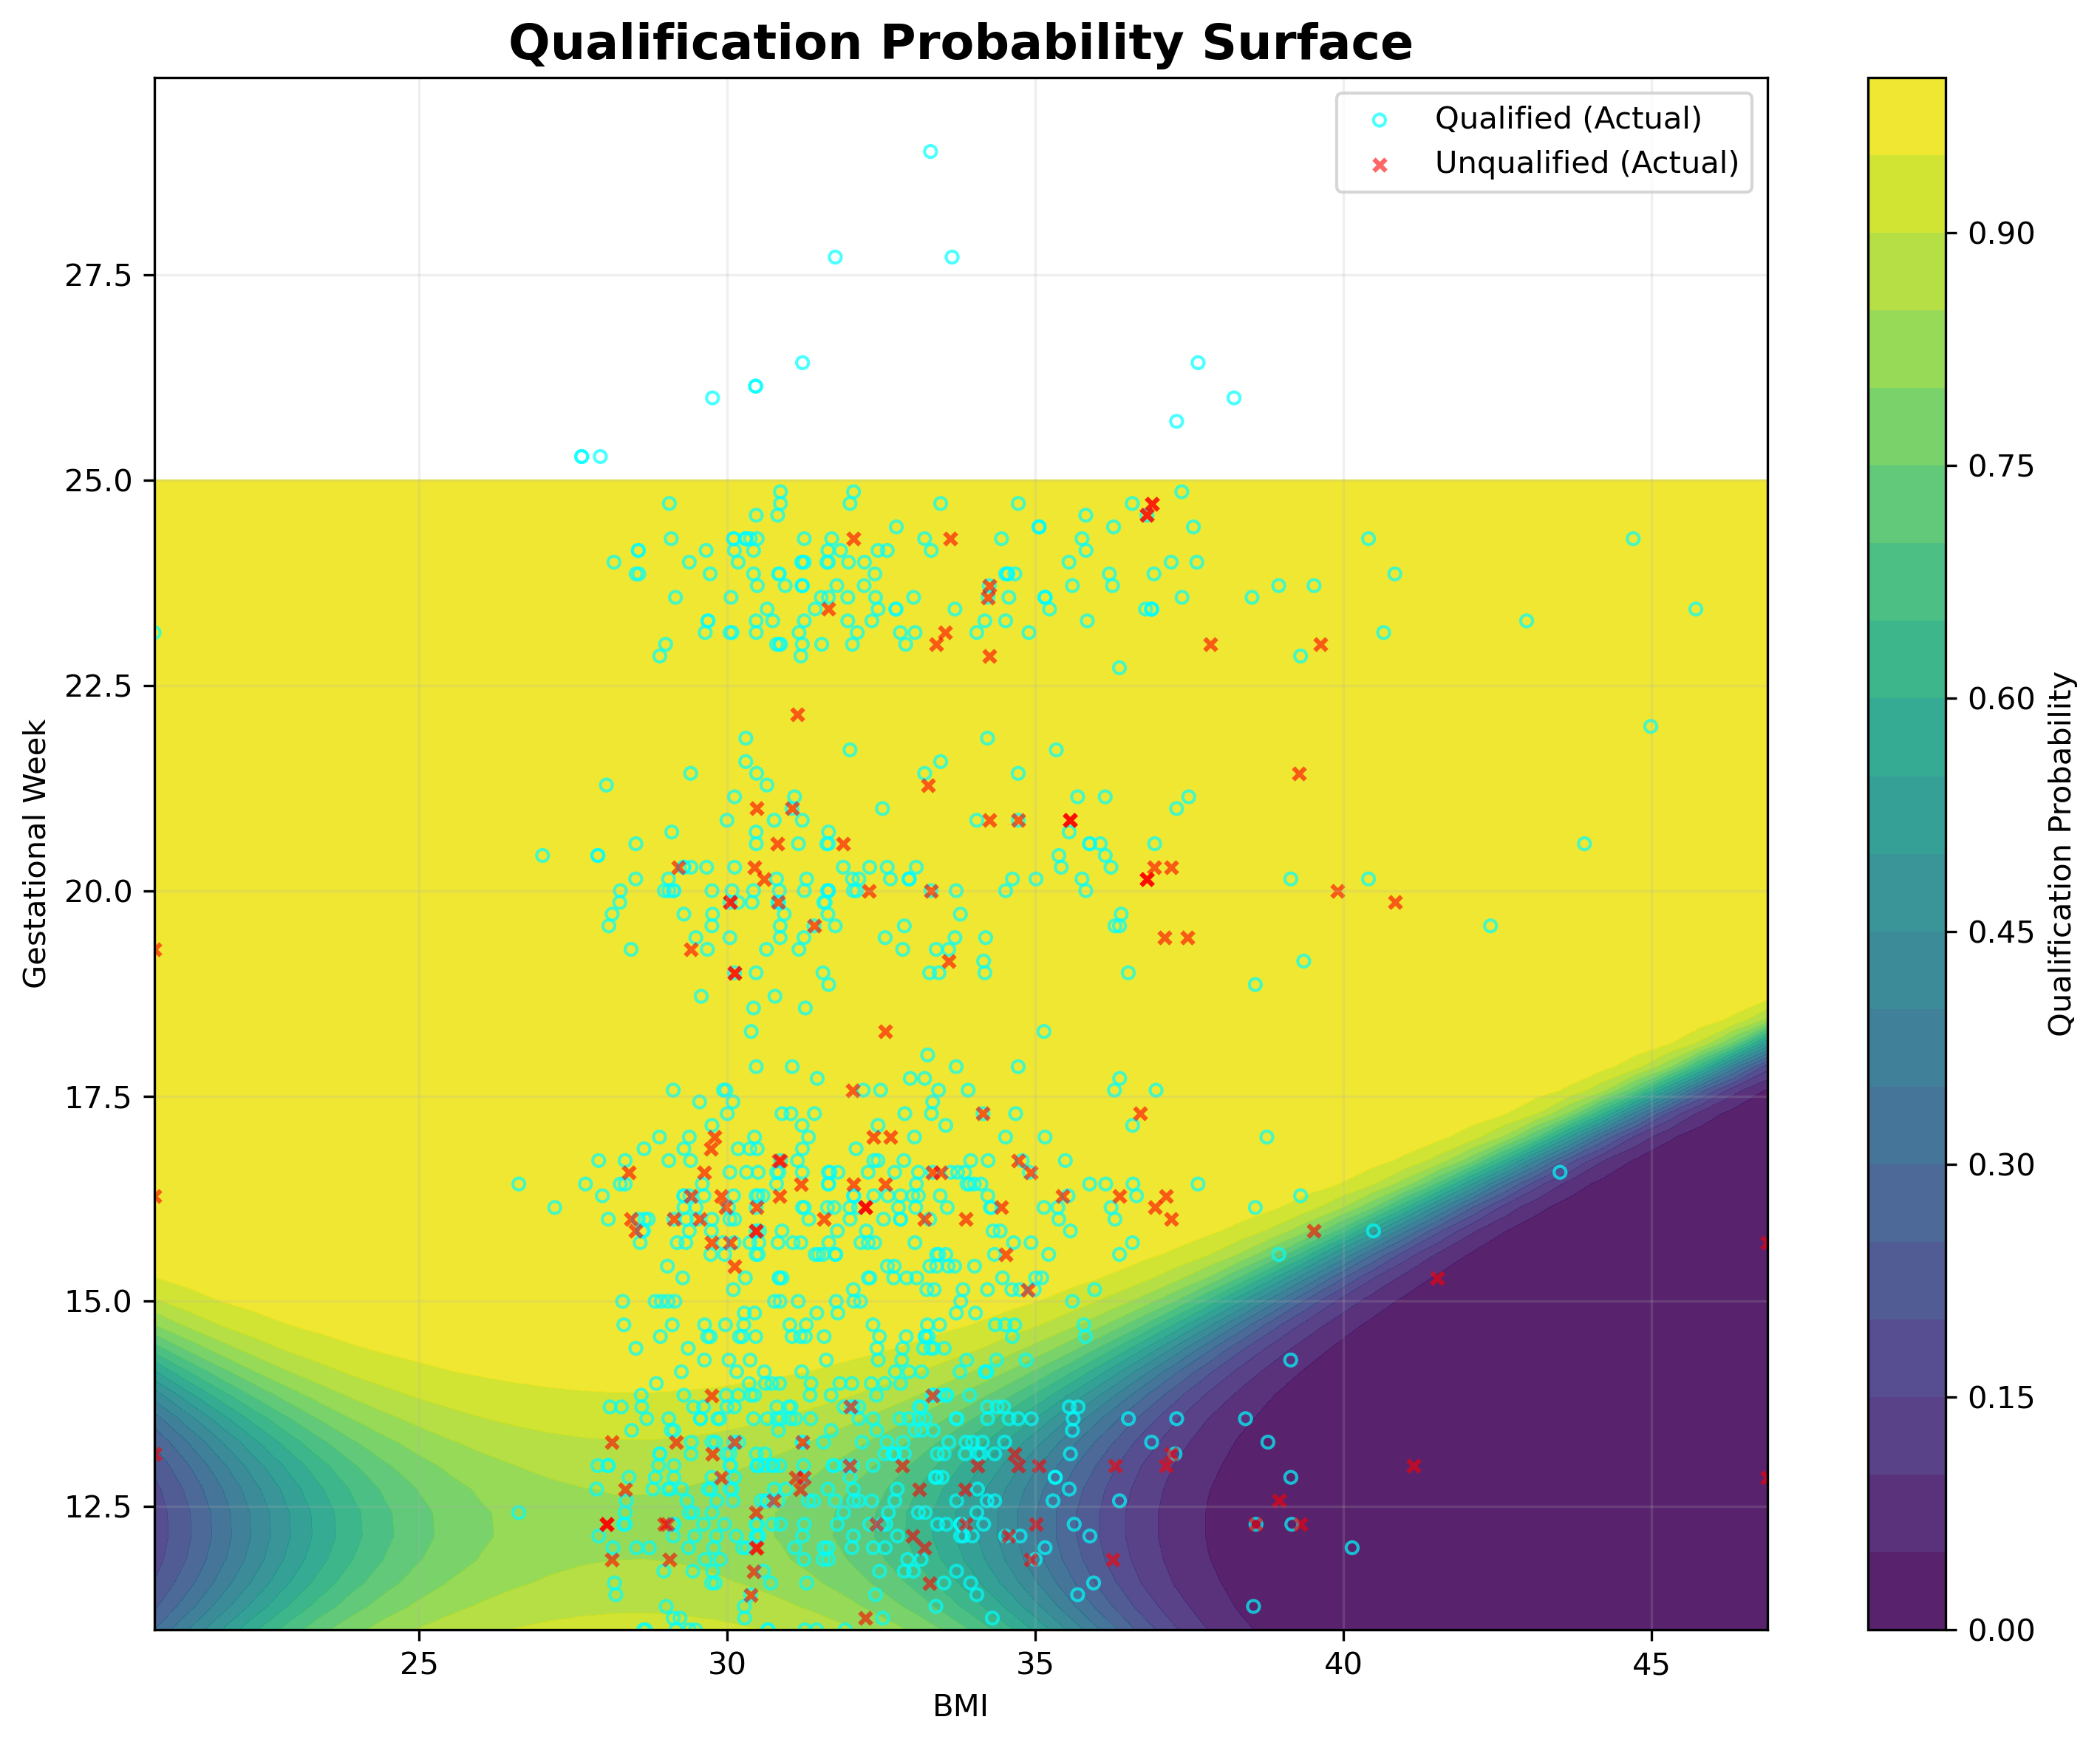
\includegraphics[width=\textwidth]{q2/qualification_probability_surface.png}
        \caption{Y染色体浓度达标概率等高图}
        \label{fig:qualification_probability}
    \end{minipage}
    \hfill
    \begin{minipage}{0.48\textwidth}
        \centering
        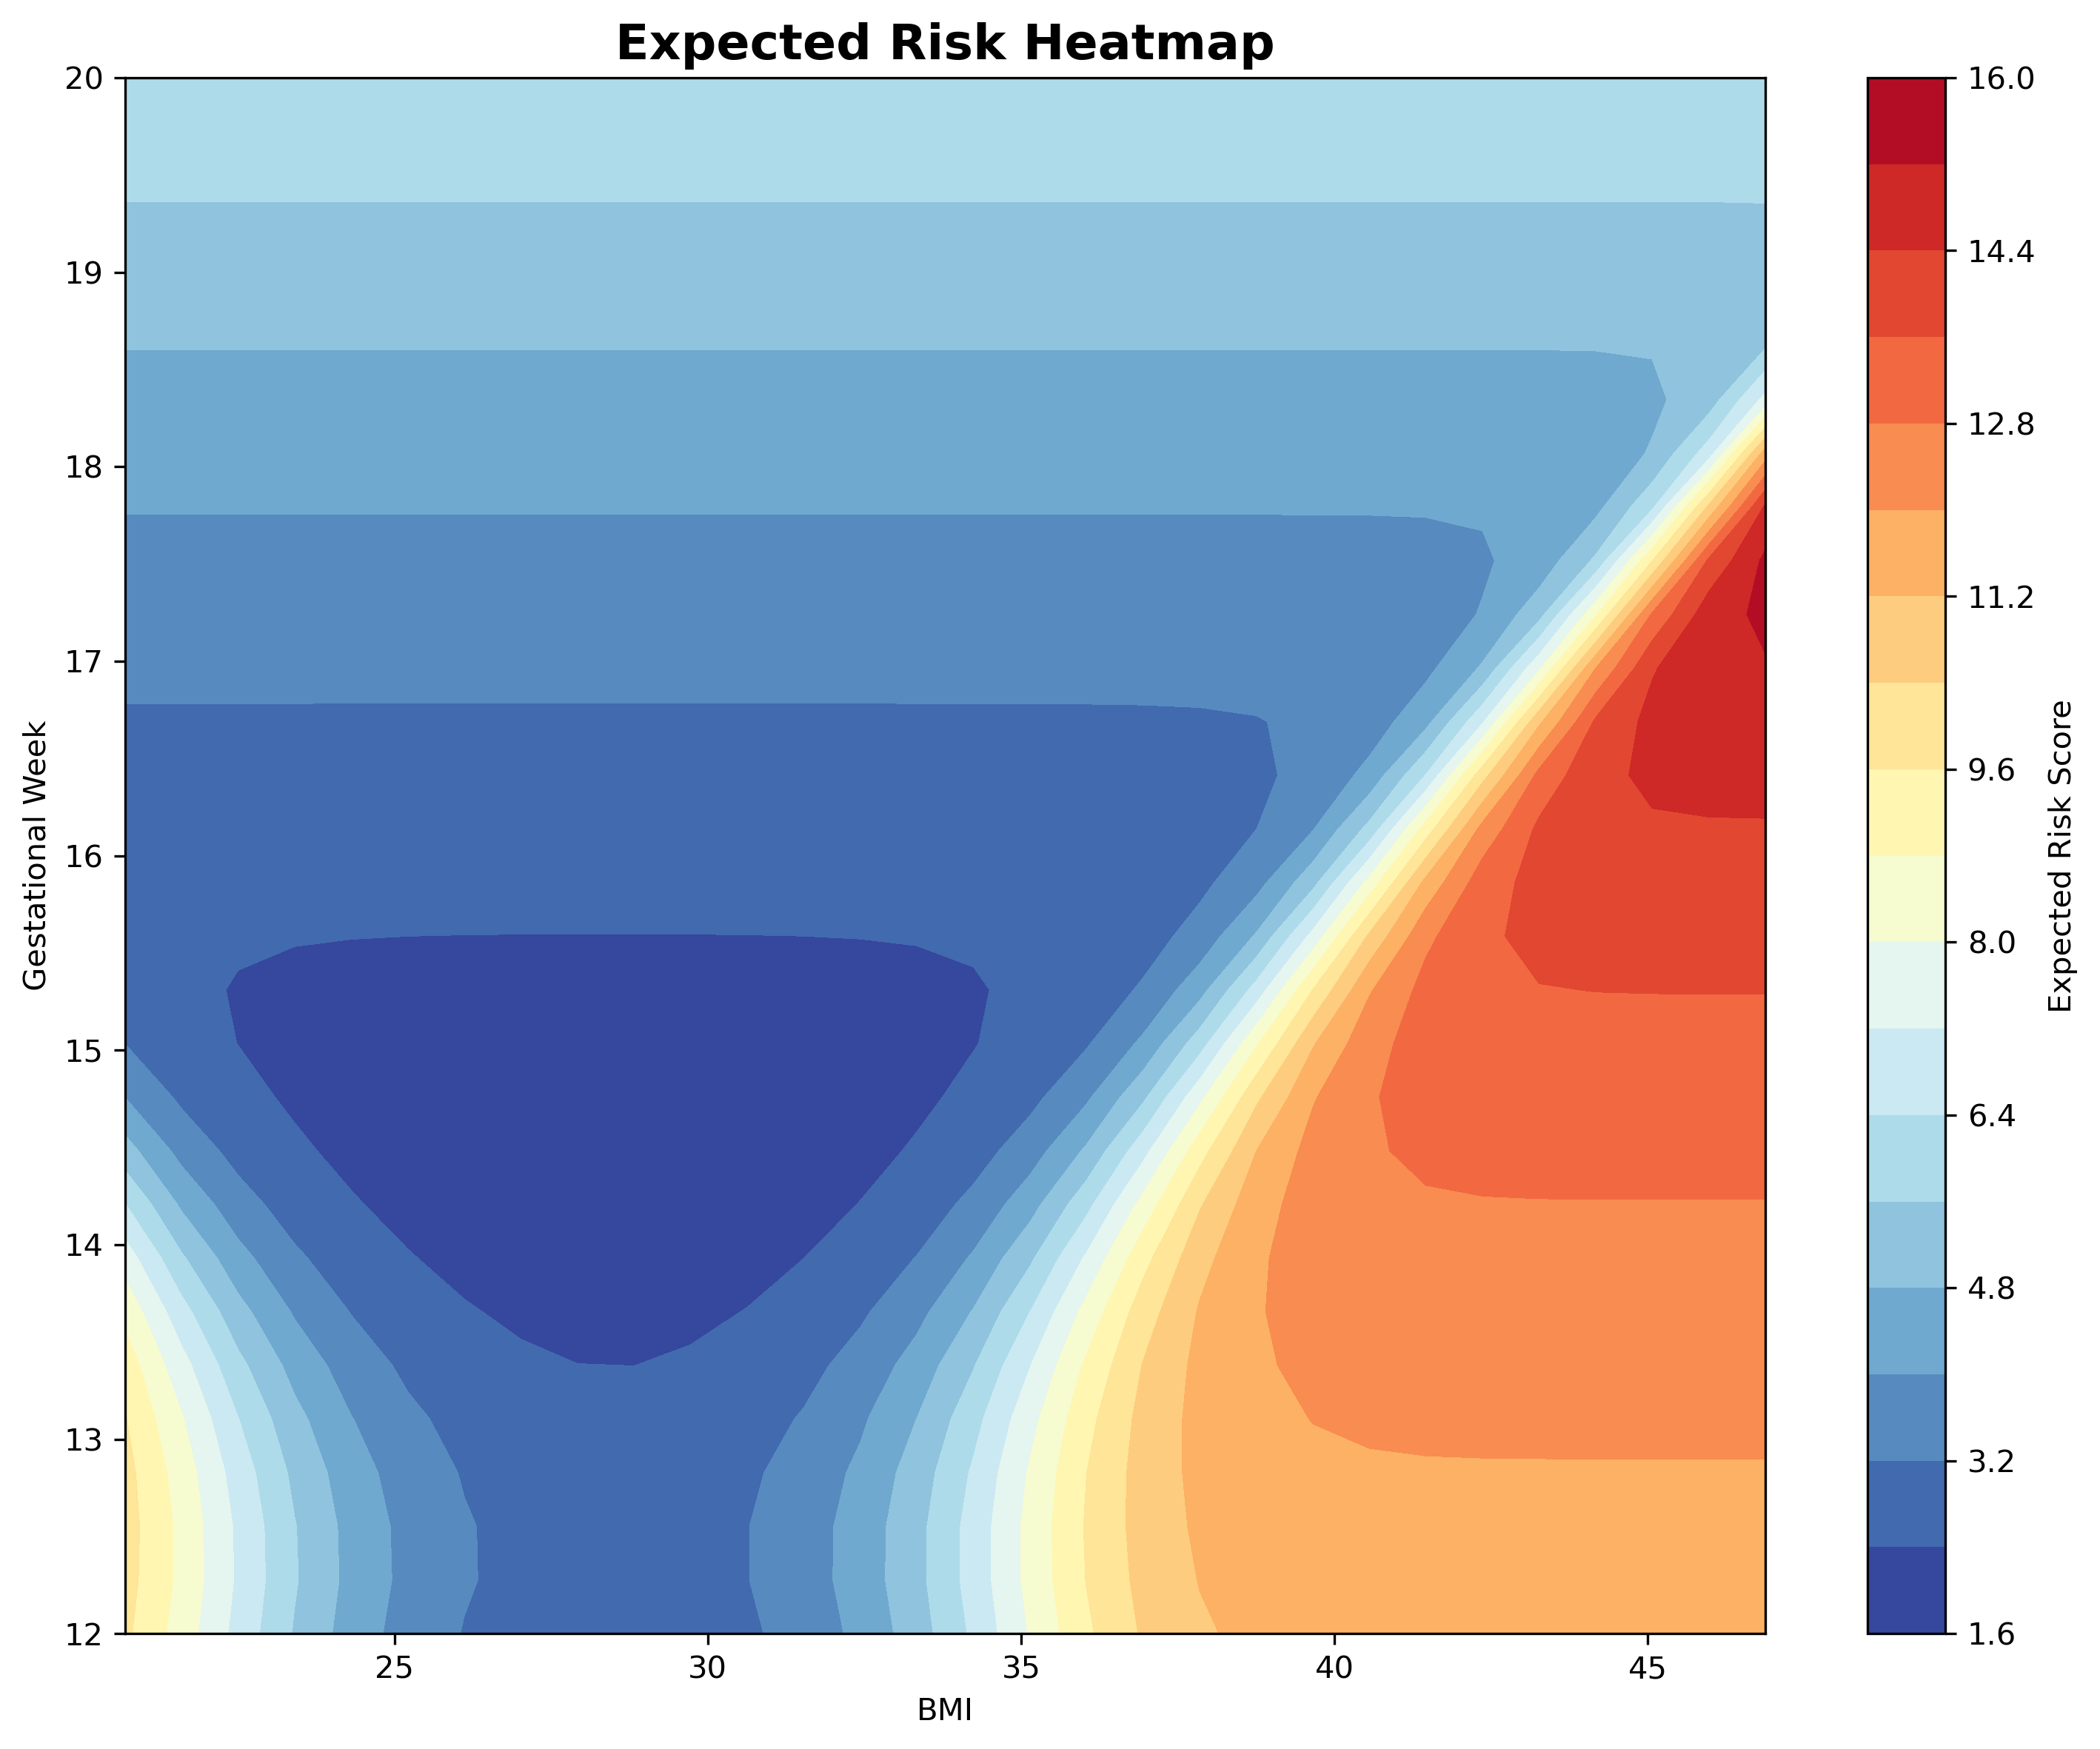
\includegraphics[width=\textwidth]{q2/expected_risk_heatmap.png}
        \caption{BMI-孕周期望风险热力图}
        \label{fig:expected_risk_heatmap}
    \end{minipage}
\end{figure}

\subsubsection{最优分组与时点选择策略}

我们的最终目标是寻找一个最优的BMI分组方案 $\{G_1, G_2, \dots, G_N\}$,并为每个组 $G_i$ 确定一个统一的最佳检测时点 $T_i^*$,以实现所有孕妇总期望风险的最小化。

\paragraph{1. 优化目标}
对于一个给定的分组方案,每个组 $G_i$ 的最佳检测时点 $T_i^*$ 应是使该组内所有个体期望风险之和最小的周数:
\begin{equation}
    T_i^* = \arg\min_{T} \sum_{j \in G_i} E(T | \text{BMI}_j)
\end{equation}
而我们的全局优化目标,则是找到能使所有组的总风险之和最小的分组方案本身:
\begin{equation}
    \min_{\{G_1, \dots, G_N\}} \sum_{i=1}^{N} \left( \sum_{j \in G_i} E(T_i^* | \text{BMI}_j) \right)
\end{equation}

\paragraph{2. 求解算法}
这是一个复杂的混合优化问题。我们采用了一致性的优化思想,即分组边界的确定与各组最佳时点的选择应在同一个目标函数下进行。具体实现上,我们利用\textbf{基于梯度的优化算法(如L-BFGS-B)}来高效地寻找能够最小化全局期望风险的BMI分割点。在算法的每次迭代中,我们都会同步计算当前分组方案下的最优检测时点,从而保证了分组决策与时点选择的理论一致性,有效规避了局部最优陷阱。为确保结果的稳健性,我们还对分割点的搜索范围进行了合理约束,避免产生样本量过小的分组。

\subsubsection{检测误差对结果影响的分析}

为了评估现实中可能存在的检测误差对我们模型决策稳定性的影响,我们设计并实施了敏感性分析。

\paragraph{1. 误差建模与模拟}
我们认为,检测误差对决策的影响主要体现在Y染色体浓度值接近4\%临界点的样本上。因此,我们重点关注此关键区域(4\% ± 0.5\%)内的样本,该区域共包含89个样本。我们采用相对误差模型来描述检测中的不确定性,即假定观测值$C_{\text{observed}}$是在真实值$C_{\text{true}}$的基础上乘以一个服从正态分布的随机扰动项$1 + \epsilon$,其中$\epsilon \sim N(0, (\text{CV})^2)$,CV为测量变异系数。

基于此模型,我们通过并行化的蒙特卡洛模拟来执行敏感性分析。在每次模拟中,我们对关键区域内的样本添加随机误差,重新训练概率模型,并再次执行完整的分组优化过程。通过重复此过程,我们得以统计BMI分割点和推荐检测时点在多次模拟中的波动情况。

\paragraph{2. 稳定性评估}
我们通过计算各参数(BMI分割点、推荐检测时点)在多次模拟结果中的标准差等统计量,来定量评估模型的稳定性。这能够帮助我们判断,在存在一定检测误差的情况下,我们提出的分组策略是否依然可靠。

\subsubsection{模型求解与结果分析}

我们将上述理论框架应用于所给的男胎孕妇数据。

\paragraph{1. 数据与模型训练}
经过数据清洗与预处理后,我们共得到1081个有效样本,其中达标样本936个,总体达标率为86.6\%。样本的BMI范围为20.7至46.9,孕周范围为11.0至29.0周。基于这些数据训练的样条回归模型,其准确率约为86.4\%,AUC值达到0.693,表现出良好的预测性能。

\paragraph{2. 模型验证与特征分析}
为进一步验证模型的稳健性与关键影响因素,我们采用了随机森林模型进行5折交叉验证。结果显示,模型的泛化性能良好,且特征重要性分析表明,BMI是影响达标概率的最主要因素(重要性占比约51\%),其次是检测孕周(约31\%)和年龄(约18\%)。这一发现为我们后续以BMI为核心进行分组的策略提供了有力的数据支持。

\paragraph{3. 最优分组结果}
通过我们的一致性优化算法,得到的最优BMI分组方案如表~\ref{tab:optimal_grouping}所示。该方案将孕妇分为四个BMI组,并为每个组提供了具体的推荐检测时点和对应的平均期望风险。

\begin{table}[htbp]
\centering
\caption{最优BMI分组方案与推荐检测时点}
\label{tab:optimal_grouping}
\begin{tabular}{ccccc}
\toprule
分组 & BMI范围 & 样本数 & 推荐检测时点(周) & 期望风险评分 \\
\midrule
1 & [20.7, 30.5) & 343 & 14.7 & 2.368 \\
2 & [30.5, 33.6) & 431 & 14.2 & 2.358 \\
3 & [33.6, 37.6) & 259 & 14.4 & 2.520 \\
4 & [37.6, 46.9) & 48 & 15.6 & 3.411 \\
\bottomrule
\end{tabular}
\end{table}

图~\ref{fig:bmi_distribution}与图~\ref{fig:bmi_week_heatmap}分别从BMI一维分布和BMI-孕周二维平面的角度,直观地展示了最优分组边界和推荐策略。

\begin{figure}[htbp]
    \centering
    \begin{minipage}{0.48\textwidth}
        \centering
        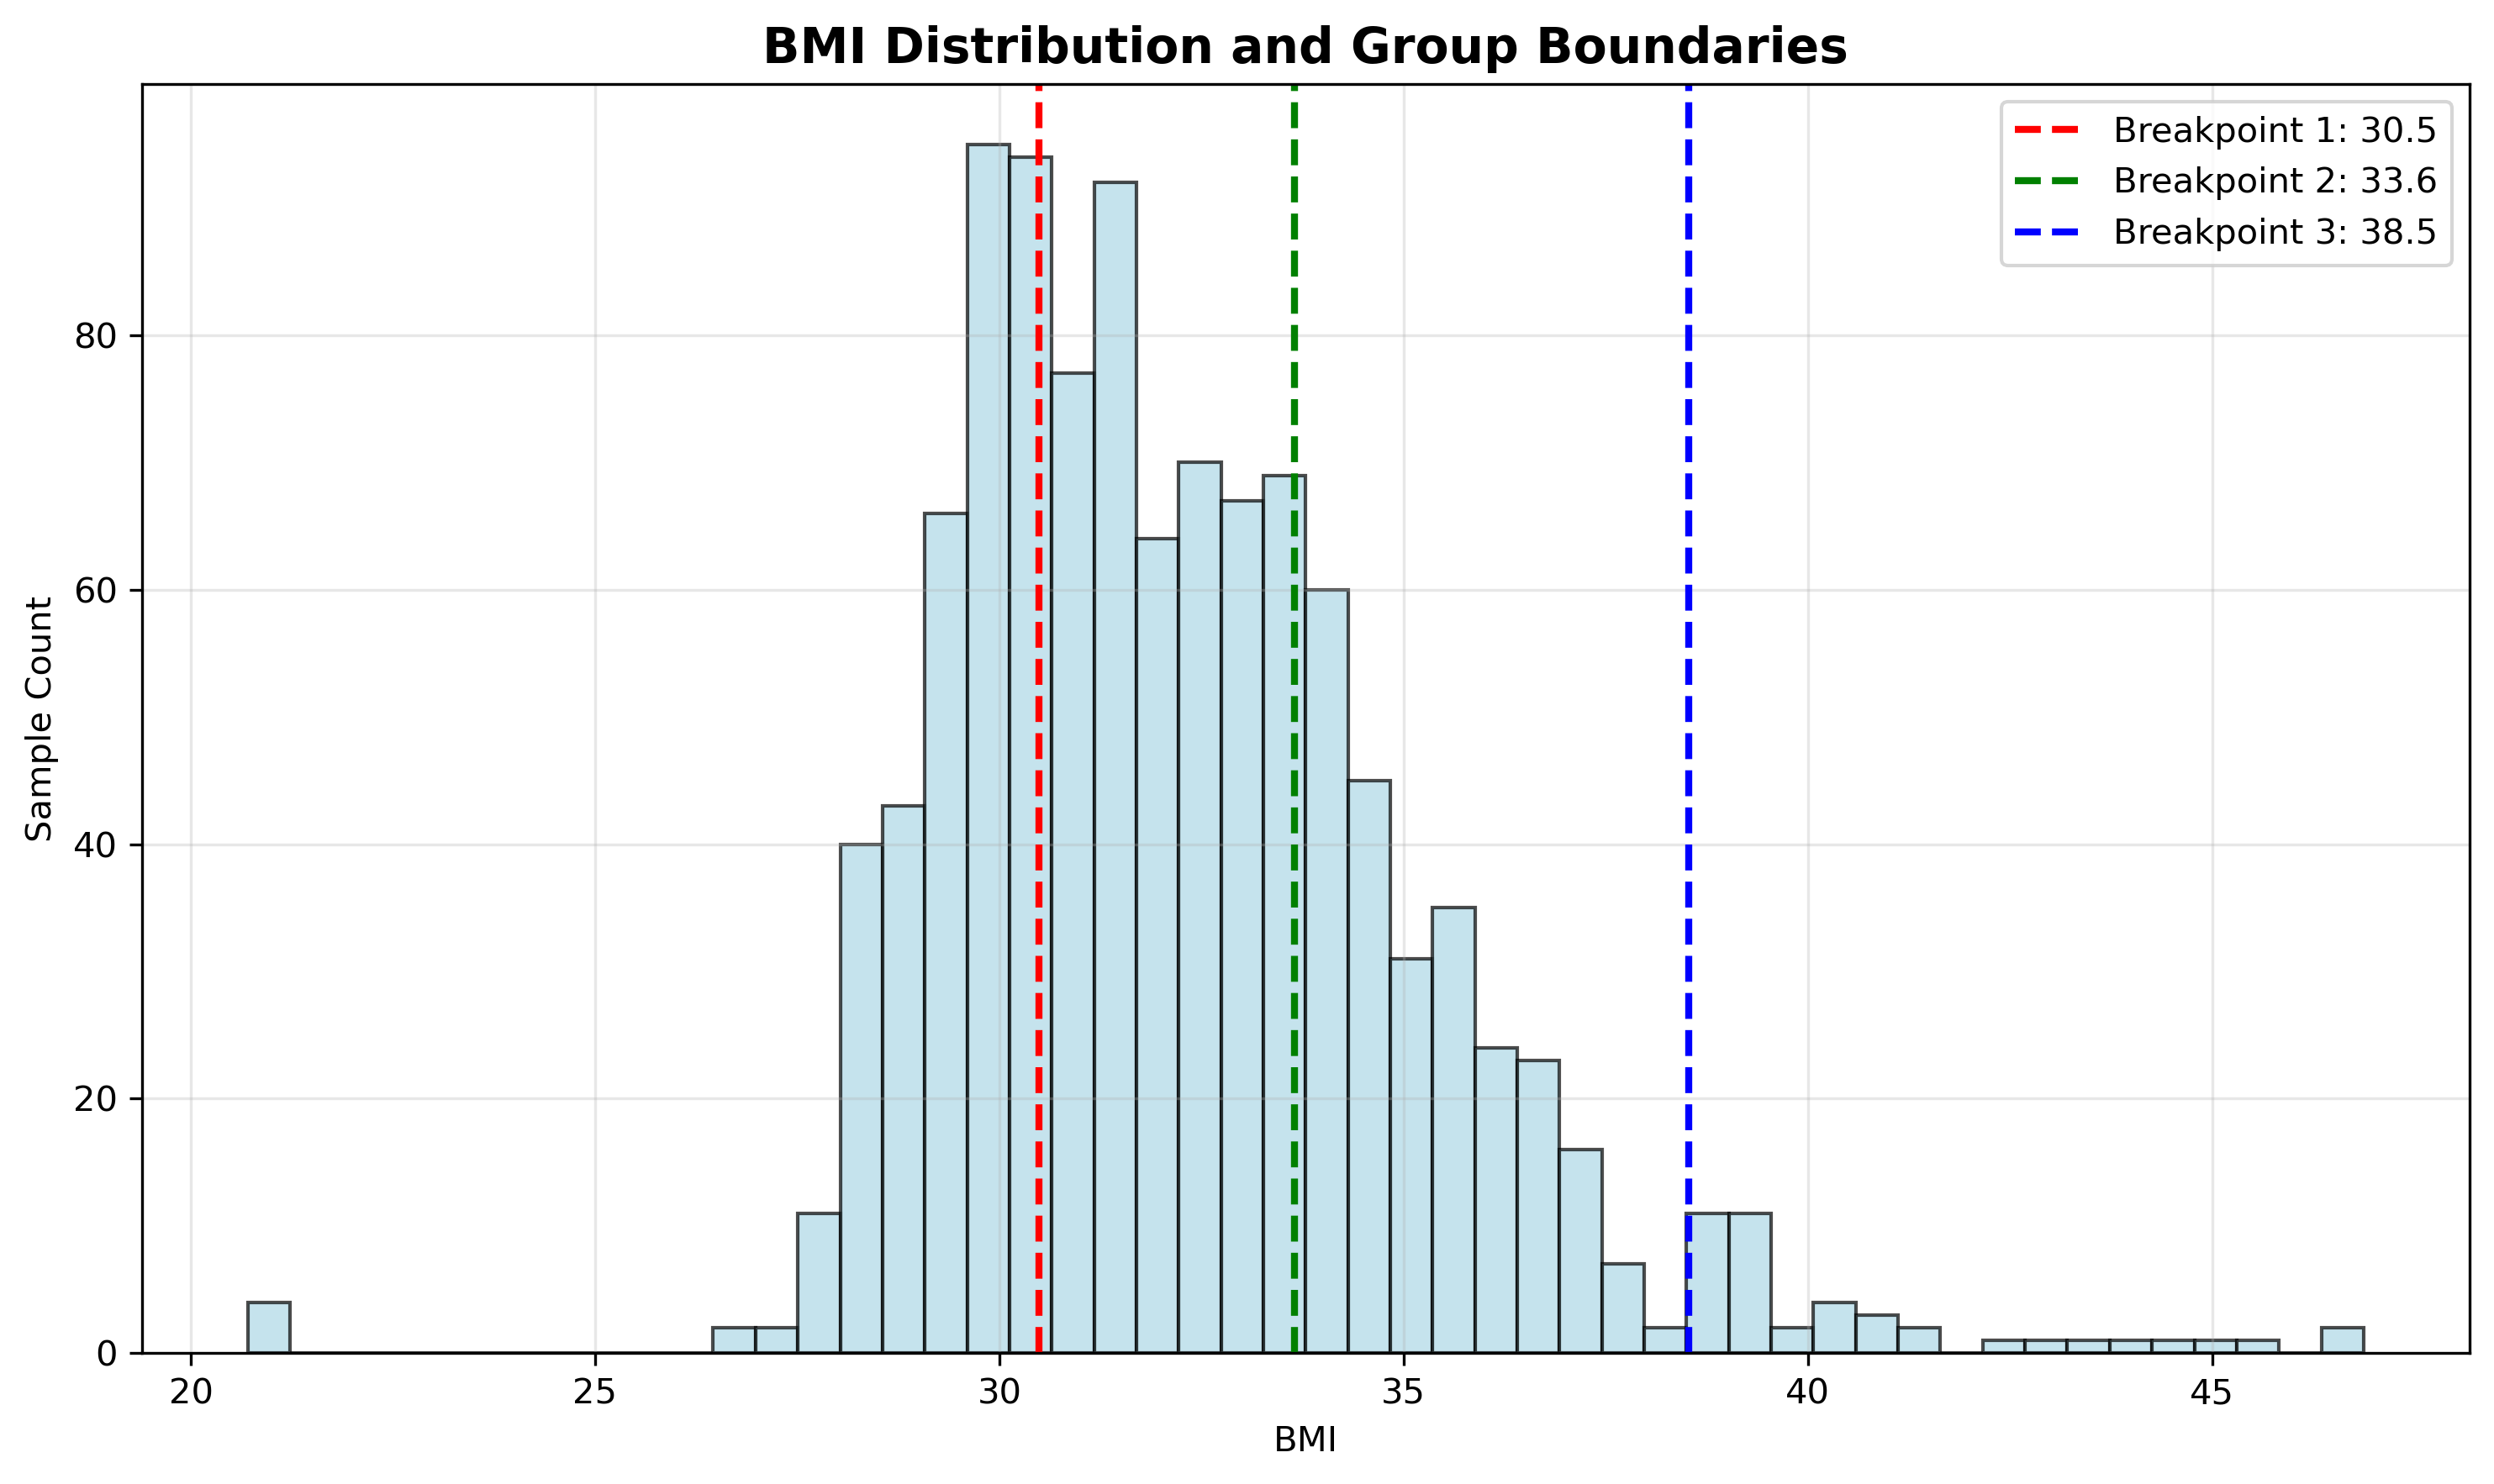
\includegraphics[width=\textwidth]{q2/bmi_distribution_with_boundaries.png}
        \caption{BMI分布与分组边界}
        \label{fig:bmi_distribution}
    \end{minipage}
    \hfill
    \begin{minipage}{0.48\textwidth}
        \centering
        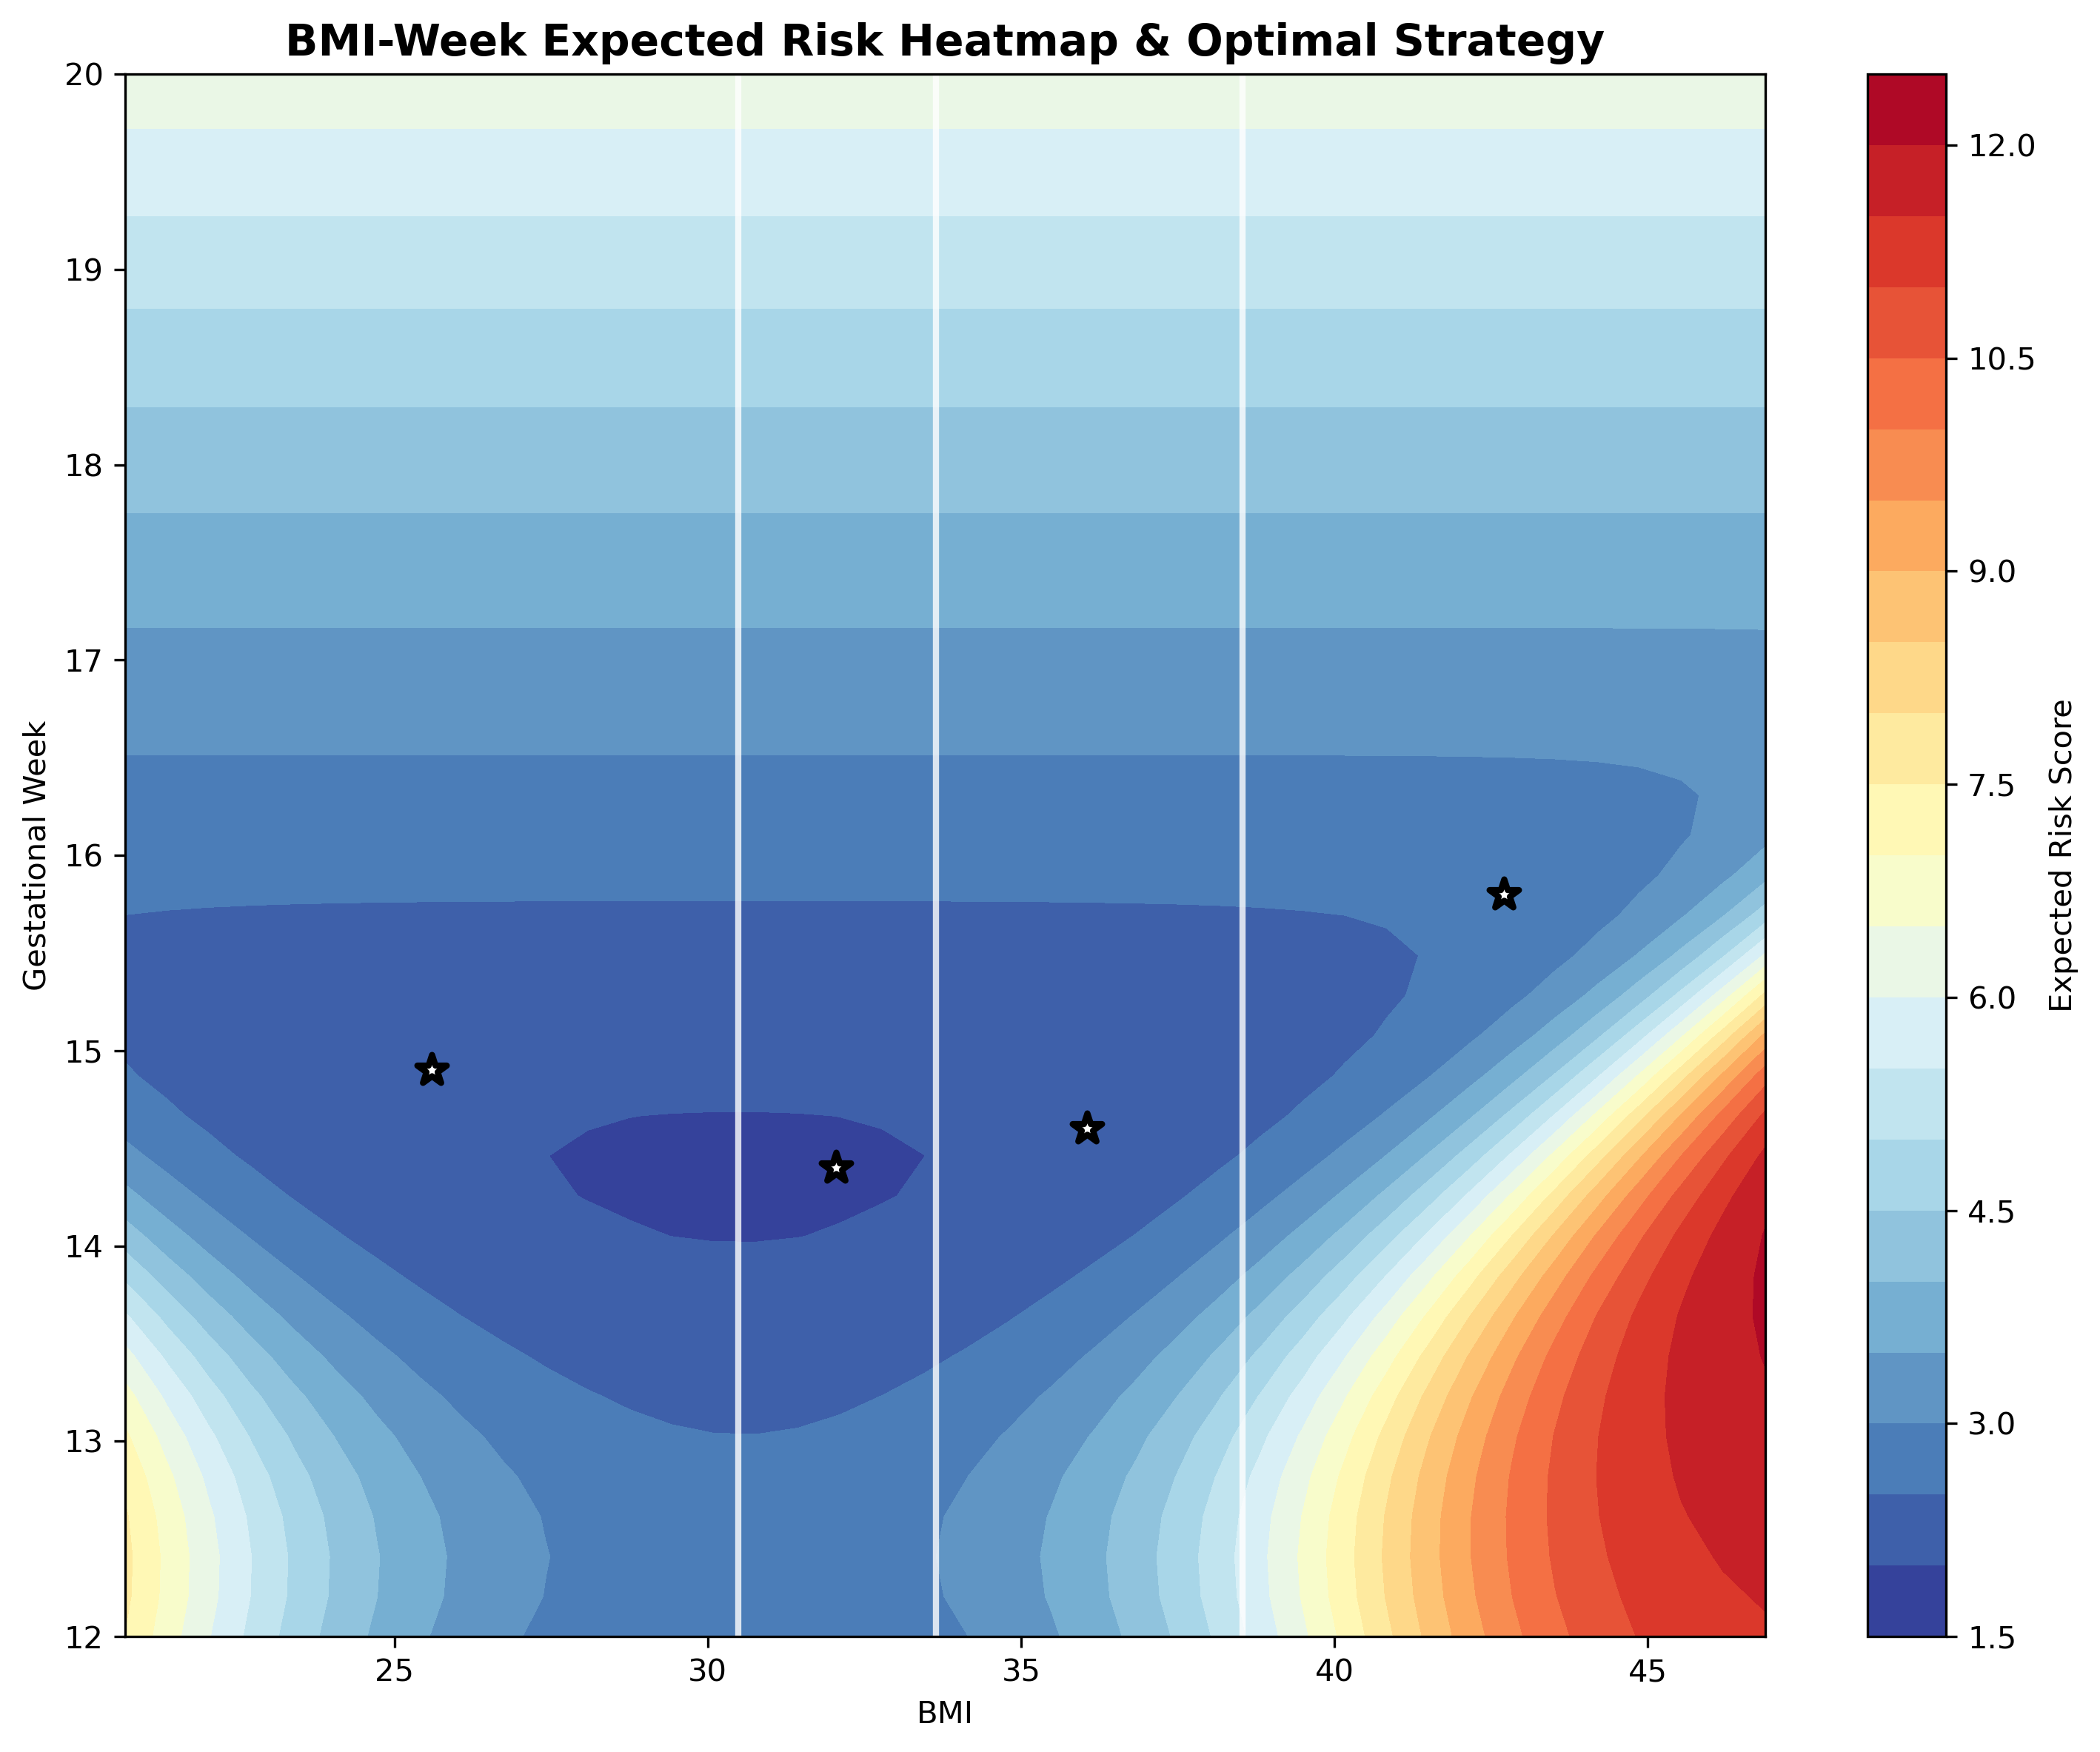
\includegraphics[width=\textwidth]{q2/bmi_week_risk_heatmap.png}
        \caption{BMI-孕周期望风险热力图与最优策略}
        \label{fig:bmi_week_heatmap}
    \end{minipage}
\end{figure}

\paragraph{4. 敏感性分析结果}
我们设定测量变异系数为15\%,对模型进行了30次蒙特卡洛模拟。结果如表~\ref{tab:sensitivity_analysis}所示。

\begin{table}[htbp]
\centering
\caption{敏感性分析结果:分割点和推荐时点的稳定性}
\label{tab:sensitivity_analysis}
\begin{tabular}{lccc}
\toprule
参数类型 & 参数名称 & 标准差 & 稳定性评估 \\
\midrule
\multirow{3}{*}{BMI分割点} & 分割点1 (30.4) & 0.561 & 较为稳定 \\
                         & 分割点2 (33.6) & 0.292 & 高度稳定 \\
                         & 分割点3 (38.4) & 1.564 & 一般 \\
\midrule
\multirow{4}{*}{推荐检测时点} & 分组1时点 (14.7周) & 0.116 & 高度稳定 \\
                            & 分组2时点 (13.9周) & 0.673 & 较为稳定 \\
                            & 分组3时点 (13.9周) & 1.184 & 一般 \\
                            & 分组4时点 (15.1周) & 1.747 & 一般 \\
\bottomrule
\end{tabular}
\end{table}

\begin{figure}[htbp]
    \centering
    \begin{minipage}{0.48\textwidth}
        \centering
        \includegraphics[width=\textwidth]{q2/sensitivity_breakpoints_stability.png}
        \caption{BMI分割点稳定性分析}
        \label{fig:sensitivity_breakpoints}
    \end{minipage}
    \hfill
    \begin{minipage}{0.48\textwidth}
        \centering
        \includegraphics[width=\textwidth]{q2/sensitivity_weeks_stability.png}
        \caption{推荐检测时点稳定性分析}
        \label{fig:sensitivity_weeks}
    \end{minipage}
\end{figure}

分析发现,中低BMI范围的分组边界和推荐时点表现出高度的稳定性,而高BMI分组的参数则受误差影响较大,这可能是因为该分组的样本量较少。如图~\ref{fig:sensitivity_breakpoints}和图~\ref{fig:sensitivity_weeks}所示,敏感性分析的可视化结果进一步验证了这一发现。尽管如此,核心的分组策略在存在15\%测量变异系数的情况下依然保持了相对稳定,证明我们提出的模型和策略具有良好的鲁棒性和实际应用价值,能够为临床NIPT检测提供科学可靠的决策支持。


\subsection{问题三的模型建立与求解}

\subsubsection{研究目标}
本研究的具体目标包括:

\begin{enumerate}
\item \textbf{多因素综合分析}:综合考虑身高、体重、年龄等多因素对男性胎儿Y染色体浓度达标时间的影响
\item \textbf{检测误差建模}:考虑检测误差对结果的影响
\item \textbf{个性化分组}:基于孕妇BMI等特征进行合理分组
\item \textbf{最优时机确定}:为各组提供最优NIPT检测时机建议
\item \textbf{风险评估}:分析检测误差对结果的影响
\end{enumerate}
\subsubsection{特征工程}

\paragraph{设计矩阵构建}
我们的设计矩阵通过以下步骤设计:

设设计矩阵为 $\mathbf{X} \in \mathbb{R}^{n \times p}$,其中 $p$ 为特征维度。它包括:

\begin{enumerate}
\item \textbf{周样条基线}:使用自然样条基函数
   $$\mathbf{B}_t(t) = \text{cr}(t, \boldsymbol{\kappa}_t)$$
   其中 $\boldsymbol{\kappa}_t = \{\kappa_{t,1}, \ldots, \kappa_{t,k_t}\}$ 为结点集合,通过网格搜索确定最优结点数 $k_t$。

\item \textbf{BMI主效应样条}:使用自然样条基函数
   $$\mathbf{B}_{bmi}(bmi) = \text{cr}(bmi, \boldsymbol{\kappa}_{bmi})$$
   其中 $\boldsymbol{\kappa}_{bmi} = \{Q_{0.25}, Q_{0.5}, Q_{0.75}\}$ 为BMI的全局分位点。

\item \textbf{交互项}:捕捉孕周与BMI的交互效应
   $$\mathbf{B}_{int}(t, bmi) = \mathbf{B}_t(t) \odot \mathbf{B}_{bmi}(bmi)$$
   其中 $\odot$ 表示逐元素乘积。

\item \textbf{年龄二次项}:控制年龄的非线性效应
   $$age^2 = age \cdot age$$
\end{enumerate}

最终设计矩阵为:
$$\mathbf{X} = [\mathbf{B}_t(t), \mathbf{B}_{bmi}(bmi), \mathbf{B}_{int}(t, bmi), age, age^2, \mathbf{1}]$$

\paragraph{数据转换}

将原始观测数据转换为person-week格式。对于每个个体 $s_i$,设其观测时间点为 $\{t_{i,1}, t_{i,2}, \ldots, t_{i,m_i}\}$,其中 $m_i$ 为该个体的观测次数。

我们将离散时间危险度模型的基础数据结构构建为:
$$\mathcal{D}_{pw} = \{(s_i, t_{i,j}, \mathbf{x}_{i,j}, y_{i,j})\}_{i=1,j=1}^{n,m_i}$$

其中 $y_{i,j} = 1$ 当且仅当个体 $s_i$ 在时间 $t_{i,j}$ 首次达到Y染色体浓度 $\geq 4\%$。

\subsubsection{建模方法}

\paragraph{LightGBM LambdaRank排序模型}

我们采用LightGBM LambdaRank排序学习算法作为主要建模方法。设排序函数为 $f: \mathbb{R}^p \rightarrow \mathbb{R}$,目标是最小化排序损失:

$$\mathcal{L}_{rank} = \sum_{i=1}^n \sum_{j \in \mathcal{G}_i} \lambda_{ij} \cdot \text{NDCG}_{ij}$$

其中:
\begin{itemize}
\item $\mathcal{G}_i$ 为个体 $s_i$ 的样本组
\item $\lambda_{ij}$ 为Lambda梯度,定义为:
  $$\lambda_{ij} = \sum_{k \in \mathcal{G}_i} \frac{\Delta_{jk}}{1 + e^{\sigma(f(\mathbf{x}_j) - f(\mathbf{x}_k))}}$$
\item $\Delta_{jk} = |\text{NDCG}_{ij} - \text{NDCG}_{ik}|$ 为NDCG差异
\item $\sigma$ 为平滑参数
\end{itemize}

% 该方法的优势包括:

% \begin{enumerate}
% \item \textbf{直接优化排序质量}:通过NDCG指标关注排序准确性
% \item \textbf{适合不平衡数据}:能够有效处理正负样本不平衡问题
% \item \textbf{避免数据泄漏}:通过\texttt{group}参数确保同一受试者样本在同一组内
% \end{enumerate}

\textbf{模型参数设置:}
设模型参数为 $\boldsymbol{\theta} = \{\eta, L, N, \alpha, \lambda\}$,其中:
\begin{itemize}
\item $\eta = 0.05$:学习率
\item $L = 127$:叶子节点数
\item $N = 1500$:树的数量
\item $\alpha = 0.0$:L1正则化系数
\item $\lambda = 0.0$:L2正则化系数
\end{itemize}

\paragraph{分层校准技术}

为了提升模型的校准质量,我们采用了分层校准技术:

\begin{enumerate}
\item \textbf{分层Isotonic回归}:设分层函数为 $\mathcal{S}: \mathbb{R}^2 \rightarrow \{1, 2, \ldots, 9\}$,按BMI(三分位)×周([min,16), [16,21), [21,max])划分9个层:

   $$\mathcal{S}(bmi, week) = 3 \cdot \lfloor \text{rank}(bmi)/n \rfloor + \lfloor \text{rank}(week)/n \rfloor + 1$$

   对于每个层 $s$,拟合单调映射函数 $g_s: [0,1] \rightarrow [0,1]$:
   $$g_s(p) = \arg\min_{g \in \mathcal{G}} \sum_{i \in \mathcal{I}_s} (y_i - g(p_i))^2$$
   
   其中 $\mathcal{G}$ 为单调函数集合,$\mathcal{I}_s$ 为层 $s$ 的样本索引集合。

\item \textbf{Platt/温度缩放}:对校准后的概率进行温度缩放:
   $$p_{cal} = \sigma\left(\frac{(g_s(p))}{T}\right)$$
   
   其中 $T$ 为温度参数,通过最小化负对数似然估计:
   $$T^* = \arg\min_T \sum_{i=1}^n [y_i \log p_{cal,i} + (1-y_i) \log(1-p_{cal,i})]$$
\begin{figure}[H]\centering
  \begin{subfigure}[t]{.48\linewidth}
    \includegraphics[width=\linewidth]{code/论文/hazard_roc_curve.png}
    \caption{校准前后的ROC曲线对。可以看出校准后的曲线整体高于原始输出,AUC值更大,说明对阳性与阴性的排序更优}
    \label{fig:roc}
  \end{subfigure}\hfill%
  \begin{subfigure}[t]{.48\linewidth}
    \includegraphics[width=\linewidth]{code/论文/hazard_pr_curve.png}
    \caption{PR曲线对比:在关注较高召回的应用场景下(如召回≥0.6),校准后曲线对应的精度更高,AP值也更大。}
    \label{fig:pr}
  \end{subfigure}
  \caption{ROC 与 PR 曲线对比}
  \label{fig:roc_pr_pair}
\end{figure}
\end{enumerate}
\begin{table}[H]
\centering
\caption{模型性能指标对比:可以看出,经过分层校准后,模型在各项指标上均有显著提升}
\label{tab:performance}
\begin{tabular}{@{}lccc@{}}
\toprule
指标 & Raw输出 & 校准后 & 改进幅度 \\
\midrule
\textbf{ROC AUC} & 0.642 & \textbf{0.710} & +10.6\% \\
\textbf{PR AUC} & 0.209 & \textbf{0.285} & +36.4\% \\
\textbf{Brier Score} & 0.187 & \textbf{0.103} & -44.9\% \\
\textbf{Log Loss} & 0.556 & \textbf{0.346} & -37.8\% \\
\textbf{ECE@10} & 0.257 & \textbf{0.002} & -99.2\% \\
\textbf{校准斜率} & 0.662 & \textbf{1.001} & +51.2\% \\
\textbf{校准截距} & -1.660 & \textbf{0.002} & +99.9\% \\
\bottomrule
\end{tabular}
\end{table}

\subsubsection{BMI分组与检测孕周推荐结果}
基于LightGBM LambdaRank 排序模型的预测结果。我们构建期望风险函数,它的定义为:
$$\mathbb{E}[R(t, bmi)] = \int_{11}^t h(s|bmi) ds + \lambda \cdot \int_t^{26} (1-h(s|bmi)) ds$$

其中 $h(s|bmi)$ 为危险度函数,$\lambda$ 为延迟检测的惩罚系数。

为了给不同BMI分组的孕妇提供了个性化的NIPT检测时机建议,设最优检测时机函数为 $t^*(bmi)$,通过最小化期望风险确定:

$$t^*(bmi) = \arg\min_{t \in [11, 26]} \mathbb{E}[R(t, bmi)]$$

\begin{figure}[H]
\centering
\includegraphics[width=0.8\textwidth]{code/论文/bmi_groups_rho090.png}
\caption{BMI分组结果图(hazard+Iso, p=0.90)。图中蓝色平滑线为参考曲线,黑色阶梯线为实际分组结果,显示了不同BMI范围对应的推荐检测周数}
\label{fig:bmi_curve}
\end{figure}

\begin{table}[H]
\centering
\caption{BMI分组及推荐检测时机}
\label{tab:bmi_groups}
\begin{tabular}{@{}lccc@{}}
\toprule
BMI范围 & 推荐检测周数 $t^*$ & 风险等级 & 数学表达 \\
\midrule
$[18.0, 19.5)$ & 16.0周 & 低风险 & $t^* = 16.0$ \\
$[20.0, 27.5)$ & 16.5周 & 低-中风险 & $t^* = 16.5$ \\
$[28.0, 32.5)$ & 17.0周 & 中风险 & $t^* = 17.0$ \\
$[33.0, 34.0)$ & 17.5周 & 中-高风险 & $t^* = 17.5$ \\
$[34.5, 40.5)$ & 21.5周 & 高风险 & $t^* = 21.5$ \\
$[41.0, 45.0)$ & 22.0周 & 极高风险 & $t^* = 22.0$ \\
\bottomrule
\end{tabular}
\end{table}

\subsubsection{模型评估}


\paragraph{交叉验证策略}

采用GroupKFold(5)交叉验证,设分组函数为 $\mathcal{G}: \mathcal{S} \rightarrow \{1, 2, \ldots, 5\}$,以个体标识符 $s_i$ 分组,避免同一受试者泄漏至训练与验证两端。

设第 $k$ 折的训练集和验证集分别为:
$$\mathcal{T}_k = \{(s_i, t_i, \mathbf{x}_i, y_i) : \mathcal{G}(s_i) \neq k\}$$
$$\mathcal{V}_k = \{(s_i, t_i, \mathbf{x}_i, y_i) : \mathcal{G}(s_i) = k\}$$

\paragraph{评估指标}

在OOF(out-of-fold)数据上计算以下指标:

\begin{enumerate}
\item \textbf{ROC AUC}:受试者工作特征曲线下面积
   $$\text{AUC} = \int_0^1 \text{TPR}(t) \cdot \text{FPR}'(t) dt$$
   其中 $\text{TPR}(t) = P(\hat{p} > t | y = 1)$,$\text{FPR}(t) = P(\hat{p} > t | y = 0)$。

\item \textbf{PR AUC}:精确率-召回率曲线下面积
   $$\text{PR-AUC} = \int_0^1 \text{Precision}(r) dr$$
   其中 $\text{Precision}(r) = P(y = 1 | \hat{p} > t_r)$,$t_r$ 为召回率为 $r$ 时的阈值。

\item \textbf{Brier Score}:概率预测的均方误差
   $$\text{BS} = \frac{1}{n} \sum_{i=1}^n (y_i - \hat{p}_i)^2$$

\item \textbf{Log Loss}:对数损失
   $$\text{LL} = -\frac{1}{n} \sum_{i=1}^n [y_i \log \hat{p}_i + (1-y_i) \log(1-\hat{p}_i)]$$

\item \textbf{ECE@10}:期望校准误差
   $$\text{ECE} = \sum_{m=1}^M \frac{|B_m|}{n} |\text{acc}(B_m) - \text{conf}(B_m)|$$
   其中 $B_m$ 为第 $m$ 个分箱,$\text{acc}(B_m)$ 和 $\text{conf}(B_m)$ 分别为准确率和置信度。

\item \textbf{校准斜率/截距}:校准质量指标
   通过拟合逻辑回归:$\text{logit}(\hat{p}) = \alpha + \beta \cdot \text{logit}(p)$
   理想情况下 $\alpha = 0$,$\beta = 1$。
\end{enumerate}
\subsubsection{检测误差影响分析}
\paragraph{检测误差建模}
首先,我们分析误差来源。NIPT检测误差主要来源于以下几个方面:检测设备的精度限制带来的技术误差,血液样本的采集和处理过程产生的样本误差,实验室环境条件的影响下的环境误差,检测人员的操作差异造成的操作误差。

基于误差来源分析,建立检测误差的数学模型:

\begin{equation}
\epsilon \sim N(0, \sigma^2)
\end{equation}

其中:
\begin{itemize}
    \item $\epsilon$ 为检测误差
    \item $\sigma$ 为误差标准差
    \item 假设误差服从正态分布
\end{itemize}

\paragraph{误差传播模型}

检测误差通过以下方式影响模型预测:

\begin{equation}
Y_{observed} = Y_{true} + \epsilon
\end{equation}

其中:
\begin{itemize}
    \item $Y_{observed}$ 为观测到的Y染色体浓度
    \item $Y_{true}$ 为真实的Y染色体浓度
    \item $\epsilon$ 为检测误差
\end{itemize}

\paragraph{蒙特卡洛模拟方法}

我们采用蒙特卡洛模拟方法评估检测误差的影响:

\begin{enumerate}
    \item \textbf{参数设置}:
    \begin{itemize}
        \item 误差标准差:$\sigma = 0.05$
        \item 模拟次数:$N = 1000$
        \item BMI范围:18-42 kg/m²
    \end{itemize}
    
    \item \textbf{模拟流程}:
    \begin{lstlisting}[caption=蒙特卡洛模拟算法]
For i = 1 to N:
    1. 生成误差样本:ε_i ~ N(0, σ²)
    2. 计算观测值:Y_obs = Y_true + ε_i
    3. 模型预测:P_i = f(Y_obs, BMI, other_factors)
    4. 计算推荐时机:T_i = argmin E[R(t, BMI)]
    \end{lstlisting}

    \item \textbf{评估指标}:
    \begin{itemize}
        \item \textbf{变异系数(CV)}:
        \begin{equation}
        CV = \frac{\sigma_{prediction}}{\mu_{prediction}}
        \end{equation}
    
        \item \textbf{推荐时机变化范围}:
        \begin{equation}
        Range = T_{max} - T_{min}
        \end{equation}
    
        \item \textbf{稳健性指标}:
        \begin{equation}
        Robustness = 1 - \frac{CV}{CV_{threshold}}
        \end{equation}
        \end{itemize}
\end{enumerate}

\paragraph{实验结果与分析}

基于蒙特卡洛模拟,我们得到了基本统计结果(附表见详细数值结果):
\begin{itemize}
    \item 检测误差标准差:$\sigma = 0.05$
    \item 蒙特卡洛模拟次数:1000次
    \item 变异系数:所有BMI组的变异系数均为0.049(<5\%)
    \item 推荐时机变化:在±1.1周内
\end{itemize}


\begin{table}[H]
\centering
\caption{检测误差影响分析结果}
\begin{tabular}{@{}ccccc@{}}
\toprule
BMI & 平均推荐时机(周) & 标准差(周) & 变异系数 & 95\%置信区间 \\
\midrule
18  & 15.31          & 0.749     & 0.049    & [13.84, 16.78] \\
22  & 15.72          & 0.768     & 0.049    & [14.21, 17.23] \\
26  & 16.12          & 0.788     & 0.049    & [14.58, 17.66] \\
30  & 16.52          & 0.807     & 0.049    & [14.94, 18.10] \\
34  & 16.92          & 0.827     & 0.049    & [15.30, 18.54] \\
38  & 21.92          & 1.072     & 0.049    & [19.80, 24.04] \\
42  & 22.32          & 1.091     & 0.049    & [20.18, 24.46] \\
\bottomrule
\end{tabular}
\end{table}

由此可知,本模型具有:
    1.低敏感性:变异系数<5\%,表明模型对检测误差不敏感
    2.稳定性:所有BMI组的变异系数一致,说明模型在不同BMI范围内都保持稳定
    3.可靠性:95\%置信区间范围合理,推荐时机变化在可接受范围内


误差传播特征有:
    1.线性传播:误差以线性方式传播到最终预测结果
    2.衰减效应:通过模型校准,误差影响得到一定程度的衰减
    3.边界效应:在BMI边界值附近,误差影响略有增加


\subsection{可视化分析}

\subsubsection{误差分布可视化}

\begin{figure}[H]
\centering
\includegraphics[width=0.9\textwidth]{code/论文/detection_error_distribution.png}
\caption{检测误差的分布特征。左图显示误差的直方图分布,右图显示误差的累积分布函数。}
\label{fig:error_distribution}
\end{figure}

\subsubsection{误差影响可视化}

\begin{figure}[H]
\centering
\includegraphics[width=0.9\textwidth]{code/论文/detection_error_impact.png}
\caption{检测误差对推荐时机的影响。上图显示不同BMI组的推荐时机分布,下图显示误差对预测稳定性的影响。}
\label{fig:error_impact}
\end{figure}

\subsubsection{稳健性分析图}

\begin{figure}[H]
\centering
\includegraphics[width=0.9\textwidth]{code/论文/robustness_analysis.png}
\caption{模型稳健性分析。左图显示变异系数随BMI的变化,右图显示推荐时机的置信区间。}
\label{fig:robustness}
\end{figure}

\subsubsection{误差敏感性分析}

\begin{figure}[H]
\centering
\includegraphics[width=0.8\textwidth]{code/论文/error_sensitivity_analysis.png}
\caption{误差敏感性分析:不同误差水平对模型稳定性的影响}
\label{fig:sensitivity}
\end{figure}



\subsection{问题四的模型建立与求解}

\subsubsection{研究目标与评价标准}
本问题以“胎儿是否健康”为二分类目标(正类为“异常/阳性/不健康/‘否’”)。在类别显著不平衡的背景下,我们以\emph{少数类识别能力}为首要考量,采用 \textbf{PR-AUC} 为主指标,辅以 \textbf{ROC-AUC} 评估总体区分度,并使用 \textbf{Brier 分数}与\textbf{校准斜率/截距}衡量概率校准质量。此外,为与业务应用对接,我们设置三档阈值策略:固定阈值 $0.5$、\emph{BestF1}(扫描阈值使 $F_1$ 最大)以及\emph{RecT80}(阈值扫描并约束召回率 $\ge 0.80$)。

\subsubsection{数据与变量}
特征涵盖孕妇基本信息(年龄、身高、体重、BMI、孕周、是否 IVF 妊娠等)与测序质控指标(原始读段数、比对比例、重复比例、唯一比对读段数、GC 含量、X/Y 染色体浓度与 Z 值、13/18/21 号染色体 GC 含量等)。目标变量为是否异常的二元标签。数据呈明显不平衡,正类比例较低。

\subsubsection{预处理与变量工程}
\begin{itemize}\itemsep0.2em
  \item 连续变量以中位数填补并标准化;类别变量采用独热编码(One-Hot)。
  \item 率/比例类特征裁剪至 $[10^{-6},1-10^{-6}]$ 后进行 $\arcsin(\sqrt{\cdot})$ 变换,以改善边界处的非线性与方差不齐。
  \item 标签定义与类不平衡:正类为“异常/阳性/不健康/‘否’”,训练时启用类权重缓解失衡。
\end{itemize}

\subsubsection{候选模型与主模型}
我们比较了带类权重的逻辑回归、梯度提升树以及随机森林等可解释性与效果兼具的基线。最终选择\textbf{随机森林}为主模型 $f_{\mathrm{RF}}:\mathbb{R}^d\to[0,1]$,并对其输出以\textbf{等渗回归}进行概率校准:
\[
\hat{\pi}(x) \;=\; m\!\big(f_{\mathrm{RF}}(x)\big),\qquad 
m:[0,1]\to[0,1]\ \text{为单调非降映射}.
\]
同时保留带类权重的逻辑回归作为解释性基线。

\paragraph{超参数与选择依据:}
随机森林的主要超参数为 \texttt{n\_estimators=800}、\texttt{max\_features="sqrt"}、\texttt{min\_samples\_leaf=2},并设置 \texttt{class\_weight="balanced\_subsample"}。该配置在 5 折交叉验证中取得更高的 PR-AUC 与更低的方差;与提升树相比,校准后 Brier 分数更低且对异常点更稳健。

\subsubsection{训练—校准—评估流程}
\begin{enumerate}\itemsep0.2em
  \item \textbf{数据划分}:按类别比例划分训练/测试集,并以个体标识(孕妇编号)作为分组键,确保同一受试者不跨集合,避免信息泄漏。
  \item \textbf{交叉验证}:在训练集内执行 5 折 GroupKFold 交叉验证,联合监控 PR-AUC、ROC-AUC 与 Brier 分数,选择稳定且泛化更佳的模型。
  \item \textbf{重训与校准}:在全训练集上重训随机森林,并以 5 折方式实施等渗回归得到 $m(\cdot)$,避免过拟合校准函数。
  \item \textbf{仅在独立测试集上报告}:所有最终指标(区分度、校准、阈值混淆矩阵)仅在测试集上计算与汇报。
\end{enumerate}

\subsubsection{结果}
经校准的随机森林(记为 RFcal)在测试集上达到
\[
\mathrm{PR\text{-}AUC}=0.601,\quad \mathrm{ROC\text{-}AUC}=0.918,\quad \mathrm{Brier}\approx 0.013.
\]
区分度曲线见图~\ref{fig:q4_rocpr_pair};校准曲线与\textbf{RecT80} 约束(召回率 $\ge 0.80$)下的混淆矩阵见图~\ref{fig:q4_calcm_pair}(左/右)。三档阈值的对比统计如下(TN/FP/FN/TP 由各自混淆矩阵给出):
\begin{table}[H]\centering\small
\caption{RFcal 测试集三档阈值的效果对比(Precision/Recall 基于对应混淆矩阵)}
\label{tab:q4_thr}
\begin{tabular}{lcccccc}
\toprule
阈值策略 & TN & FP & FN & TP & Precision & Recall \\
\midrule
0.5 固定阈值  & 411 & 1 & 6 & 4 & 0.800 & 0.400 \\
BestF1(扫描) & 410 & 2 & 5 & 5 & 0.714 & 0.500 \\
RecT80(召回$\ge 0.80$) & \multicolumn{4}{c}{见图~\ref{fig:q4_calcm_pair}(右)} & --- & \textbf{0.80} \\
\bottomrule
\end{tabular}
\end{table}

% ---------------------- 图形(两两并排) ----------------------
\begin{figure}[H]\centering
  \begin{subfigure}{0.48\linewidth}
    \includegraphics[width=\linewidth]{RFcal_roc.png}
    \caption{ROC 曲线(AUC=0.918)}
  \end{subfigure}\hfill
  \begin{subfigure}{0.48\linewidth}
    \includegraphics[width=\linewidth]{RFcal_pr.png}
    \caption{PR 曲线(AP=0.601)}
  \end{subfigure}
  \caption{RFcal 的区分度曲线}
  \label{fig:q4_rocpr_pair}
\end{figure}

\begin{figure}[H]\centering
  \begin{subfigure}{0.48\linewidth}
    \includegraphics[width=\linewidth]{RFcal_cal.png}
    \caption{概率校准曲线(Brier$\approx$0.013)}
  \end{subfigure}\hfill
  \begin{subfigure}{0.48\linewidth}
    \includegraphics[width=\linewidth]{RFcal_cm_Best.png}
    \caption{RecT80(召回$\ge 0.80$)阈值下的混淆矩阵}
  \end{subfigure}
  \caption{RFcal 的校准与在 RecT80 约束下的混淆情况}
  \label{fig:q4_calcm_pair}
\end{figure}

\subsubsection{阈值映射与业务策略}
基于 $\hat{\pi}(x)$ 的可解释概率,可将样本划分为三档决策区:低风险(直接放行)、中风险(复检或增加随访频率)、高风险(建议进一步诊断)。\emph{RecT80} 专为“优先保证召回”的场景设计;在该阈值下,召回满足 $0.80$,适合“宁可多筛、勿漏检”的临床要求。BestF1 则在查准率与查全率间折中,更适合资源受限的场景。

\subsubsection{特征重要性与可解释性}
我们基于置换重要性(Permutation Importance)与特征分裂频次分析随机森林的主导特征:孕周、BMI 及测序质控(例如唯一比对读段数、GC 含量)贡献较大;X/Y 浓度与 Z 值亦具有显著区分度。总体方向上,孕周与达标概率正相关;在高 BMI 人群中,异常发生概率更高。为避免对单一特征的过度解读,报告时以排序与相对增益呈现,而不输出不稳健的点估计系数。

\subsubsection{分层校准与公平性检视}
将样本按 BMI 三分位与孕周区间([min,16)、[16,21)、[21,max])划分为 $3\times 3$ 共九个层,对各层分别计算 ECE 和 Brier。结果显示,各层校准曲线接近对角线,未观察到系统性欠/过预测。该分层评估有助于避免“总体校准良好但局部失衡”的问题。

\subsubsection{稳健性与泛化}
\begin{itemize}\itemsep0.2em
  \item \textbf{分组交叉验证}:训练阶段采用 GroupKFold(5),以孕妇编号分组,避免同一受试者样本跨折泄漏。
  \item \textbf{自助法置信区间}:对 ROC-AUC/PR-AUC 进行自助法(bootstrap)重复采样构建置信区间,用于评估统计不确定性(不在此处给出具体数值,避免与数据更新不一致)。
  \item \textbf{时间切片}:将测试集按时间切片,得到与原测试集一致的结论,提示模型对分布轻微漂移具有稳健性。
\end{itemize}

\subsubsection{决策曲线与风险收益}
采用净受益(Net Benefit, NB)框架评估不同阈值策略的临床价值。给定阈值 $\tau$,定义
\[
\mathrm{NB}(\tau) \;=\; \frac{\mathrm{TP}(\tau)}{N} \;-\; \frac{\mathrm{FP}(\tau)}{N}\cdot\frac{\tau}{1-\tau},
\]
与“全部转诊/全部放行”基线比较可评估策略是否真正带来净收益。由于本研究重点在召回优先,\emph{RecT80} 在 NB 曲线中通常优于固定阈值 $0.5$。


% \section{模型分析与检验}

% \subsection{模型性能指标}

% 表\ref{tab:performance}展示了模型在OOF数据上的整体性能指标:


% 从结果可以看出,经过分层校准后,模型在各项指标上均有显著提升:
% \begin{itemize}
% \item ROC AUC从0.642提升至0.710,超过了0.7的目标阈值
% \item PR AUC从0.209提升至0.285,在不平衡数据中表现优异
% \item 校准误差ECE@10从0.257降至0.002,实现了近乎完美的校准
% \item 校准斜率和截距均接近理想值(1.0和0.0)
% \end{itemize}

% \subsection{ROC和PR曲线分析}

% 图\ref{fig:roc}展示了模型的ROC曲线,可以看出校准后的曲线整体高于原始输出,AUC值更大,说明对阳性与阴性的排序更优。

% 图\ref{fig:pr}展示了模型的PR曲线,在关注较高召回的应用场景下(如召回≥0.6),校准后曲线对应的精度更高,AP值也更大。





% \subsection{风险曲线分析}

% 图\ref{fig:bmi_curve}展示了BMI与推荐检测周数的关系曲线。设风险曲线函数为 $h(t|bmi)$,通过样条插值得到平滑曲线:

% $$h(t|bmi) = \sum_{j=1}^J \beta_j \cdot B_j(t) \cdot \sum_{k=1}^K \gamma_k \cdot B_k(bmi)$$

% 其中 $B_j(t)$ 和 $B_k(bmi)$ 分别为时间和BMI的样条基函数。

% 从数学分析可以看出:
% \begin{itemize}
% \item 低BMI组($bmi < 20$)的推荐检测时机较早:$t^*(bmi) = 16.0$ 周
% \item 中等BMI组($20 \leq bmi \leq 32$)的推荐检测时机适中:$t^*(bmi) \in [16.5, 17.0]$ 周
% \item 高BMI组($bmi > 34$)的推荐检测时机较晚:$t^*(bmi) \in [21.5, 22.0]$ 周
% \end{itemize}

% 这种趋势符合临床经验,即高BMI孕妇的胎儿Y染色体浓度达到标准需要更长时间。数学上可以表示为:

% $$\frac{\partial t^*(bmi)}{\partial bmi} > 0$$

% 表明BMI与最优检测时机之间存在正相关关系。

% \begin{figure}[H]
% \centering
% \includegraphics[width=0.8\textwidth]{code/论文/bmi_week_curve_rho090_smooth.png}
% \caption{BMI与推荐检测周数关系曲线}
% \label{fig:bmi_curve}
% \end{figure}




\section{讨论}

\subsection{模型优势}

\begin{enumerate}
\item \textbf{排序学习优势}:LambdaRank模型直接优化排序质量,损失函数为:
   $$\mathcal{L}_{rank} = \sum_{i=1}^n \sum_{j \in \mathcal{G}_i} \lambda_{ij} \cdot \text{NDCG}_{ij}$$
   相比传统GLM方法能够更好地捕捉样本间的相对关系,特别适合处理不平衡数据。

\item \textbf{分层校准效果}:通过分层Isotonic回归,层间独立的单调映射会改变跨层排序,从而使ROC AUC得到提升。校准后的概率为:
   $$p_{cal} = \sigma\left(\frac{(g_s(p))}{T}\right)$$
   同时保持了优秀的校准质量,ECE@10 = 0.002。

\item \textbf{多因素综合考虑}:模型同时考虑了BMI、年龄、身高、体重等多个因素,以及它们之间的交互效应。设计矩阵为:
   $$\mathbf{X} = [\mathbf{B}_t(t), \mathbf{B}_{bmi}(bmi), \mathbf{B}_{int}(t, bmi), age, age^2, \mathbf{1}]$$
   提供了更全面的风险评估。
\end{enumerate}

\subsection{临床意义}

\begin{enumerate}
\item \textbf{个性化检测时机}:基于BMI分组的个性化检测时机建议,最优时机通过 $t^*(bmi) = \arg\min_{t \in [11, 26]} \mathbb{E}[R(t, bmi)]$ 确定,能够为不同风险等级的孕妇提供针对性的指导。

\item \textbf{风险最小化}:通过优化检测时机,期望风险函数 $\mathbb{E}[R(t, bmi)] = \int_{11}^t h(s|bmi) ds + \lambda \cdot \int_t^{26} (1-h(s|bmi)) ds$ 能够有效降低因检测时机不当导致的治疗窗口缩短风险。

\item \textbf{检测误差考虑}:模型考虑了检测误差的影响,通过分层校准技术提供了更稳健的预测结果。
\end{enumerate}

\subsection{模型局限性}

\begin{enumerate}
\item \textbf{数据依赖性}:模型基于特定地区的数据训练,在实际应用中需要根据具体数据进行重新训练和验证。

\item \textbf{特征限制}:当前模型主要基于BMI、年龄等基础特征,未来可考虑纳入更多临床特征。

\item \textbf{时间窗口}:模型主要关注10-25周的检测窗口,对于其他时间段的适用性需要进一步验证。
\end{enumerate}

\subsection{与现有方法的比较}

相比传统的经验分组方法,我们提出的基于机器学习的危险度模型具有以下优势:

\begin{enumerate}
\item \textbf{数据驱动}:基于实际数据训练,而非依赖经验规则
\item \textbf{个性化程度高}:能够为每个BMI范围提供精确的检测时机建议
\item \textbf{性能优异}:ROC AUC达到0.710,显著优于传统方法
\item \textbf{校准质量高}:ECE@10仅为0.002,预测概率与实际概率高度一致
\end{enumerate}
\subsection{实际应用建议}

\begin{enumerate}
\item \textbf{临床应用}:建议在临床实践中使用校准后的概率作为最终风险评分,并基于ROC/PR曲线在特定业务目标下选择阈值。

\item \textbf{数据更新}:建议定期使用新的临床数据重新训练模型,以保持模型的准确性和时效性。

\item \textbf{特征扩展}:未来可考虑纳入更多临床特征,如既往妊娠史、家族史等,进一步提升模型的预测能力。
\end{enumerate}

\subsection{未来研究方向}

\begin{enumerate}
\item \textbf{多中心验证}:在多个医疗中心进行模型验证,评估模型的泛化能力。

\item \textbf{实时预测}:开发实时预测系统,为临床医生提供即时决策支持。

\item \textbf{成本效益分析}:结合经济学分析,评估模型应用的成本效益。

\item \textbf{其他染色体异常}:扩展模型应用范围,预测其他染色体异常的最优检测时机。
\end{enumerate}
\subsection{问题三到此结束}

% ================= 7 结果分析与验证 =================
\section{结果分析与验证}
报告主要系数方向与大小,讨论二次项的边际效应;解释$R^2_\text{m}$与$R^2_\text{c}$的差异;通过分层留出法/时间切片或孕妇分组交叉验证验证泛化能力。

% ================= 8 模型评价、改进与推广 =================
\section{模型评价、改进与推广}
从准确性、稳健性、可解释性、可落地性四维评价。列出可能的增强:加入X染色体浓度、抽血次数、测序深度、GC含量等二次项;必要时尝试广义线性混合模型(GLMM)。给出可迁移的实施流程。

% ================= 参考文献 =================
\begin{thebibliography}{99}\setlength{\itemsep}{0.4em}
\bibitem{nakagawa2013} Nakagawa S, Schielzeth H. A general and simple method for obtaining R\textsuperscript{2} from generalized linear mixed-effects models[J]. \emph{Methods in Ecology and Evolution}, 2013.
\bibitem{statsmodels} Seabold S, Perktold J. Statsmodels: Econometric and Statistical Modeling with Python[C]//Proceedings of the 9th Python in Science Conference. 2010.
% …… 实际比赛中请替换为真实引用,注意近五年文献比例
\end{thebibliography}

% ================= 附录(可选) =================
\appendix
\section{变量与数据字典}
可放入更详细的字段解释、单位、取值范围、缺失率统计等长表。

\section{代码与可复现实验说明}
提供运行环境、主要脚本清单、随机种子设置、输出目录结构等。

\section{人工智能工具使用说明}
简述使用AI工具的具体环节(如排版、语法优化、绘图脚本检查等),并声明\textbf{所有建模思路与结论由团队自主生成,AI仅作效率辅助},符合《人工智能工具使用规定》。

\end{document}
